\documentclass[twoside]{book}

% Packages required by doxygen
\usepackage{calc}
\usepackage{doxygen}
\usepackage{graphicx}
\usepackage[utf8]{inputenc}
\usepackage{makeidx}
\usepackage{multicol}
\usepackage{multirow}
\usepackage{textcomp}
\usepackage[table]{xcolor}

% Font selection
\usepackage[T1]{fontenc}
\usepackage{mathptmx}
\usepackage[scaled=.90]{helvet}
\usepackage{courier}
\usepackage{amssymb}
\usepackage{sectsty}
\renewcommand{\familydefault}{\sfdefault}
\allsectionsfont{%
  \fontseries{bc}\selectfont%
  \color{darkgray}%
}
\renewcommand{\DoxyLabelFont}{%
  \fontseries{bc}\selectfont%
  \color{darkgray}%
}

% Page & text layout
\usepackage{geometry}
\geometry{%
  a4paper,%
  top=2.5cm,%
  bottom=2.5cm,%
  left=2.5cm,%
  right=2.5cm%
}
\tolerance=750
\hfuzz=15pt
\hbadness=750
\setlength{\emergencystretch}{15pt}
\setlength{\parindent}{0cm}
\setlength{\parskip}{0.2cm}
\makeatletter
\renewcommand{\paragraph}{%
  \@startsection{paragraph}{4}{0ex}{-1.0ex}{1.0ex}{%
    \normalfont\normalsize\bfseries\SS@parafont%
  }%
}
\renewcommand{\subparagraph}{%
  \@startsection{subparagraph}{5}{0ex}{-1.0ex}{1.0ex}{%
    \normalfont\normalsize\bfseries\SS@subparafont%
  }%
}
\makeatother

% Headers & footers
\usepackage{fancyhdr}
\pagestyle{fancyplain}
\fancyhead[LE]{\fancyplain{}{\bfseries\thepage}}
\fancyhead[CE]{\fancyplain{}{}}
\fancyhead[RE]{\fancyplain{}{\bfseries\leftmark}}
\fancyhead[LO]{\fancyplain{}{\bfseries\rightmark}}
\fancyhead[CO]{\fancyplain{}{}}
\fancyhead[RO]{\fancyplain{}{\bfseries\thepage}}
\fancyfoot[LE]{\fancyplain{}{}}
\fancyfoot[CE]{\fancyplain{}{}}
\fancyfoot[RE]{\fancyplain{}{\bfseries\scriptsize Generated on Tue Nov 24 2015 18\-:09\-:28 for Scene Graph by Doxygen }}
\fancyfoot[LO]{\fancyplain{}{\bfseries\scriptsize Generated on Tue Nov 24 2015 18\-:09\-:28 for Scene Graph by Doxygen }}
\fancyfoot[CO]{\fancyplain{}{}}
\fancyfoot[RO]{\fancyplain{}{}}
\renewcommand{\footrulewidth}{0.4pt}
\renewcommand{\chaptermark}[1]{%
  \markboth{#1}{}%
}
\renewcommand{\sectionmark}[1]{%
  \markright{\thesection\ #1}%
}

% Indices & bibliography
\usepackage{natbib}
\usepackage[titles]{tocloft}
\setcounter{tocdepth}{3}
\setcounter{secnumdepth}{5}
\makeindex

% Hyperlinks (required, but should be loaded last)
\usepackage{ifpdf}
\ifpdf
  \usepackage[pdftex,pagebackref=true]{hyperref}
\else
  \usepackage[ps2pdf,pagebackref=true]{hyperref}
\fi
\hypersetup{%
  colorlinks=true,%
  linkcolor=blue,%
  citecolor=blue,%
  unicode%
}

% Custom commands
\newcommand{\clearemptydoublepage}{%
  \newpage{\pagestyle{empty}\cleardoublepage}%
}


%===== C O N T E N T S =====

\begin{document}

% Titlepage & ToC
\hypersetup{pageanchor=false}
\pagenumbering{roman}
\begin{titlepage}
\vspace*{7cm}
\begin{center}%
{\Large Scene Graph }\\
\vspace*{1cm}
{\large Generated by Doxygen 1.8.6}\\
\vspace*{0.5cm}
{\small Tue Nov 24 2015 18:09:28}\\
\end{center}
\end{titlepage}
\clearemptydoublepage
\tableofcontents
\clearemptydoublepage
\pagenumbering{arabic}
\hypersetup{pageanchor=true}

%--- Begin generated contents ---
\chapter{Hierarchical Index}
\section{Class Hierarchy}
This inheritance list is sorted roughly, but not completely, alphabetically\-:\begin{DoxyCompactList}
\item \contentsline{section}{Camera}{\pageref{classCamera}}{}
\item \contentsline{section}{Face}{\pageref{classFace}}{}
\item \contentsline{section}{Light}{\pageref{classLight}}{}
\item \contentsline{section}{Node}{\pageref{classNode}}{}
\begin{DoxyCompactList}
\item \contentsline{section}{Animation\-Node}{\pageref{classAnimationNode}}{}
\item \contentsline{section}{Attribute\-Node}{\pageref{classAttributeNode}}{}
\item \contentsline{section}{Camera\-Node}{\pageref{classCameraNode}}{}
\item \contentsline{section}{Geom\-Node}{\pageref{classGeomNode}}{}
\item \contentsline{section}{Light\-Node}{\pageref{classLightNode}}{}
\item \contentsline{section}{Object\-Node}{\pageref{classObjectNode}}{}
\item \contentsline{section}{Transform\-Node}{\pageref{classTransformNode}}{}
\end{DoxyCompactList}
\item \contentsline{section}{Scene\-Graph}{\pageref{classSceneGraph}}{}
\item \contentsline{section}{Token\-Pair}{\pageref{structTokenPair}}{}
\item \contentsline{section}{Transform}{\pageref{classTransform}}{}
\item \contentsline{section}{Trimesh}{\pageref{classTrimesh}}{}
\item \contentsline{section}{Trimesh\-Loader}{\pageref{classTrimeshLoader}}{}
\item \contentsline{section}{Vertex}{\pageref{classVertex}}{}
\end{DoxyCompactList}

\chapter{Class Index}
\section{Class List}
Here are the classes, structs, unions and interfaces with brief descriptions\-:\begin{DoxyCompactList}
\item\contentsline{section}{\hyperlink{classAnimationNode}{Animation\-Node} }{\pageref{classAnimationNode}}{}
\item\contentsline{section}{\hyperlink{classAttributeNode}{Attribute\-Node} }{\pageref{classAttributeNode}}{}
\item\contentsline{section}{\hyperlink{classCamera}{Camera} }{\pageref{classCamera}}{}
\item\contentsline{section}{\hyperlink{classCameraNode}{Camera\-Node} }{\pageref{classCameraNode}}{}
\item\contentsline{section}{\hyperlink{classFace}{Face} }{\pageref{classFace}}{}
\item\contentsline{section}{\hyperlink{classGeomNode}{Geom\-Node} }{\pageref{classGeomNode}}{}
\item\contentsline{section}{\hyperlink{classLight}{Light} }{\pageref{classLight}}{}
\item\contentsline{section}{\hyperlink{classLightNode}{Light\-Node} }{\pageref{classLightNode}}{}
\item\contentsline{section}{\hyperlink{classNode}{Node} }{\pageref{classNode}}{}
\item\contentsline{section}{\hyperlink{classObjectNode}{Object\-Node} }{\pageref{classObjectNode}}{}
\item\contentsline{section}{\hyperlink{classSceneGraph}{Scene\-Graph} }{\pageref{classSceneGraph}}{}
\item\contentsline{section}{\hyperlink{structTokenPair}{Token\-Pair} }{\pageref{structTokenPair}}{}
\item\contentsline{section}{\hyperlink{classTransform}{Transform} }{\pageref{classTransform}}{}
\item\contentsline{section}{\hyperlink{classTransformNode}{Transform\-Node} }{\pageref{classTransformNode}}{}
\item\contentsline{section}{\hyperlink{classTrimesh}{Trimesh} }{\pageref{classTrimesh}}{}
\item\contentsline{section}{\hyperlink{classTrimeshLoader}{Trimesh\-Loader} }{\pageref{classTrimeshLoader}}{}
\item\contentsline{section}{\hyperlink{classVertex}{Vertex} }{\pageref{classVertex}}{}
\end{DoxyCompactList}

\chapter{Class Documentation}
\hypertarget{classAnimationNode}{\section{Animation\-Node Class Reference}
\label{classAnimationNode}\index{Animation\-Node@{Animation\-Node}}
}


{\ttfamily \#include $<$Animation\-Node.\-h$>$}

Inheritance diagram for Animation\-Node\-:\begin{figure}[H]
\begin{center}
\leavevmode
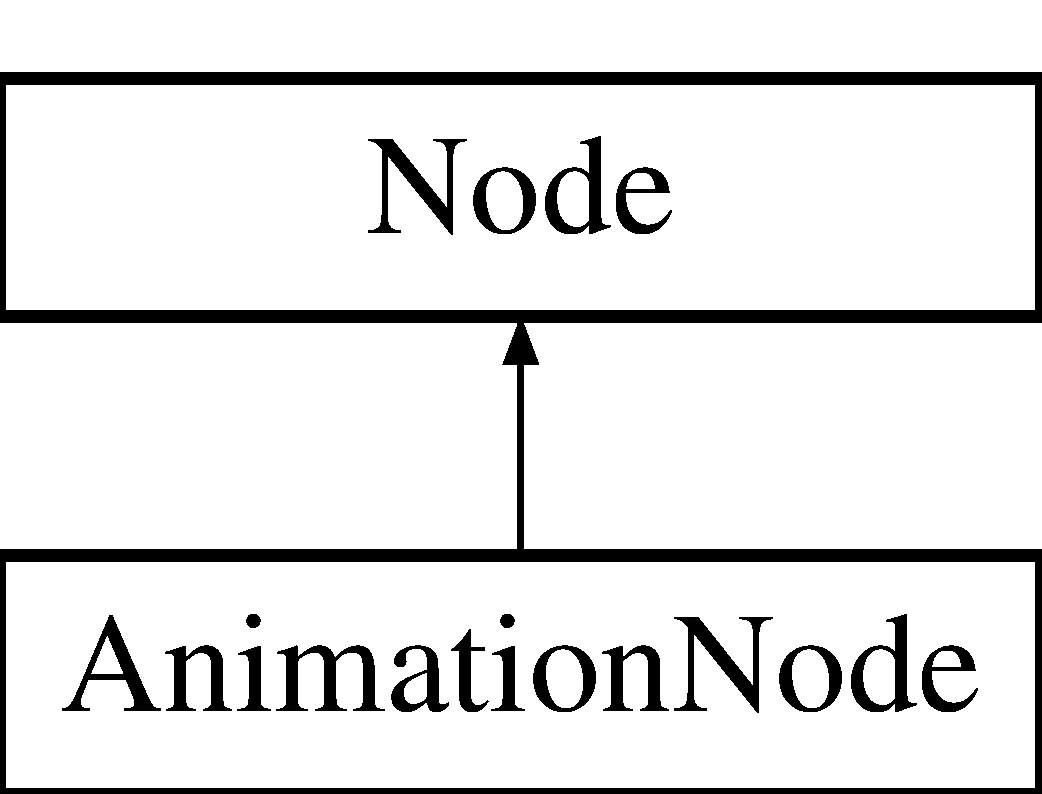
\includegraphics[height=2.000000cm]{classAnimationNode}
\end{center}
\end{figure}
\subsection*{Public Member Functions}
\begin{DoxyCompactItemize}
\item 
\hypertarget{classAnimationNode_aba1bf01dcd4f64e57ed5de4d95098269}{{\bfseries Animation\-Node} (const \hyperlink{classTransform}{Transform} \&t, const float c\-T)}\label{classAnimationNode_aba1bf01dcd4f64e57ed5de4d95098269}

\item 
void \hyperlink{classAnimationNode_a0b0bb275a3f89f45aedd35f41f459f9f}{execute} ()
\item 
\hypertarget{classAnimationNode_af03e7eef1324f9eedbfa0fc4c225f5de}{void {\bfseries set\-Parameters} (const Transform\-Type, const G\-Lfloat $\ast$a, const float c\-T)}\label{classAnimationNode_af03e7eef1324f9eedbfa0fc4c225f5de}

\end{DoxyCompactItemize}
\subsection*{Additional Inherited Members}


\subsection{Detailed Description}
Purpose\-: Class which handles the animation within the Scene Graph \begin{DoxyAuthor}{Author}
Andrew Dang-\/\-Tran This node animates all it's children with a linearly interpolated transform over time. 
\end{DoxyAuthor}


\subsection{Member Function Documentation}
\hypertarget{classAnimationNode_a0b0bb275a3f89f45aedd35f41f459f9f}{\index{Animation\-Node@{Animation\-Node}!execute@{execute}}
\index{execute@{execute}!AnimationNode@{Animation\-Node}}
\subsubsection[{execute}]{\setlength{\rightskip}{0pt plus 5cm}void Animation\-Node\-::execute (
\begin{DoxyParamCaption}
{}
\end{DoxyParamCaption}
)\hspace{0.3cm}{\ttfamily [virtual]}}}\label{classAnimationNode_a0b0bb275a3f89f45aedd35f41f459f9f}
Interpolates the transform according to the current clock time. Then multiplies the transform to the current matrix. 

Reimplemented from \hyperlink{classNode_a6890991303fcc6c9b2b3dec678c8b5db}{Node}.



The documentation for this class was generated from the following files\-:\begin{DoxyCompactItemize}
\item 
Animation\-Node.\-h\item 
Animation\-Node.\-c++\end{DoxyCompactItemize}

\hypertarget{classAttributeNode}{\section{Attribute\-Node Class Reference}
\label{classAttributeNode}\index{Attribute\-Node@{Attribute\-Node}}
}


{\ttfamily \#include $<$Attribute\-Node.\-h$>$}

Inheritance diagram for Attribute\-Node\-:\begin{figure}[H]
\begin{center}
\leavevmode
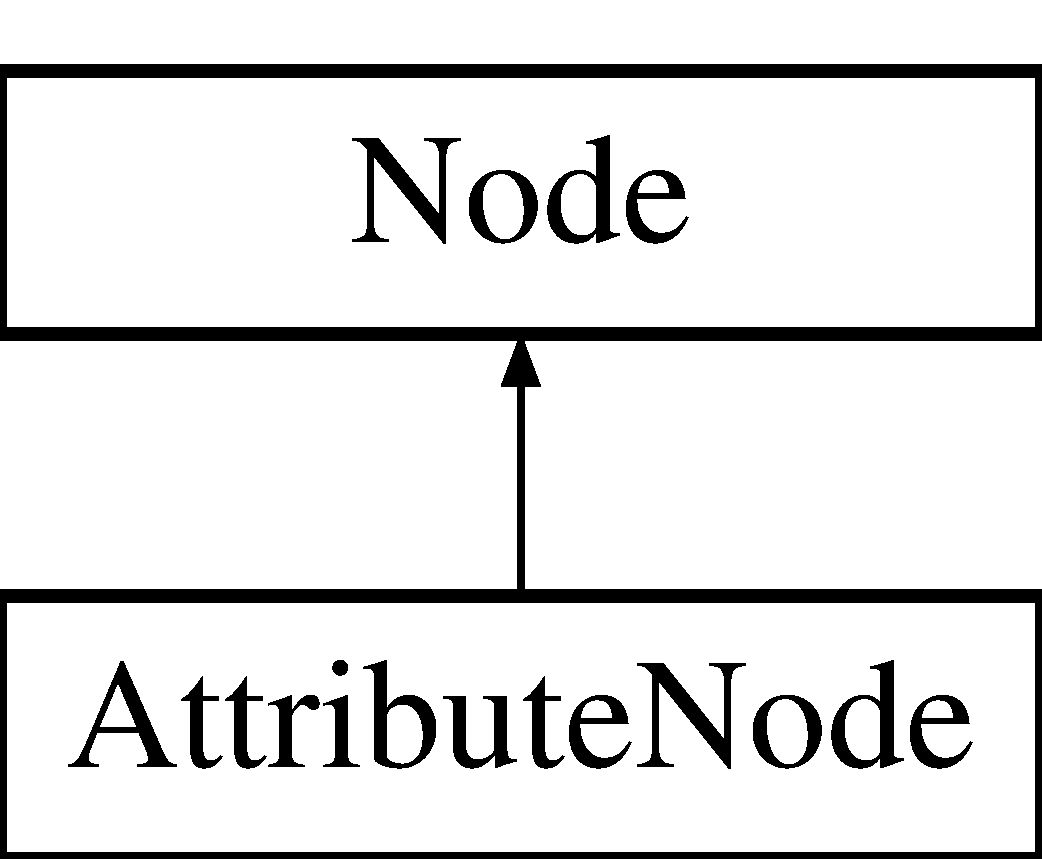
\includegraphics[height=2.000000cm]{classAttributeNode}
\end{center}
\end{figure}
\subsection*{Public Member Functions}
\begin{DoxyCompactItemize}
\item 
\hypertarget{classAttributeNode_a77f9865bfac60b16c51c046c2320935a}{{\bfseries Attribute\-Node} (const Mode m)}\label{classAttributeNode_a77f9865bfac60b16c51c046c2320935a}

\item 
void \hyperlink{classAttributeNode_ad6fb6f07dc9728e066c769c35c321f25}{execute} ()
\item 
\hypertarget{classAttributeNode_a740c689f2c62400b83cbd8b70fc9117d}{void {\bfseries set\-Parameters} (const Mode m)}\label{classAttributeNode_a740c689f2c62400b83cbd8b70fc9117d}

\end{DoxyCompactItemize}
\subsection*{Additional Inherited Members}


\subsection{Detailed Description}
This node determines the rendering mode of all of it's children. 

\subsection{Member Function Documentation}
\hypertarget{classAttributeNode_ad6fb6f07dc9728e066c769c35c321f25}{\index{Attribute\-Node@{Attribute\-Node}!execute@{execute}}
\index{execute@{execute}!AttributeNode@{Attribute\-Node}}
\subsubsection[{execute}]{\setlength{\rightskip}{0pt plus 5cm}void Attribute\-Node\-::execute (
\begin{DoxyParamCaption}
{}
\end{DoxyParamCaption}
)\hspace{0.3cm}{\ttfamily [virtual]}}}\label{classAttributeNode_ad6fb6f07dc9728e066c769c35c321f25}
Sets the correct Open\-G\-L parameters for each mode 

Reimplemented from \hyperlink{classNode_a6890991303fcc6c9b2b3dec678c8b5db}{Node}.



The documentation for this class was generated from the following files\-:\begin{DoxyCompactItemize}
\item 
Attribute\-Node.\-h\item 
Attribute\-Node.\-c++\end{DoxyCompactItemize}

\hypertarget{classCamera}{\section{Camera Class Reference}
\label{classCamera}\index{Camera@{Camera}}
}


{\ttfamily \#include $<$Camera.\-h$>$}

\subsection*{Public Member Functions}
\begin{DoxyCompactItemize}
\item 
\hypertarget{classCamera_a61d3ad16da64ac0f6d465c216269e105}{{\bfseries Camera} (const G\-Lfloat $\ast$pos, const G\-Lfloat $\ast$subject\-Pos, const G\-Lfloat n, const G\-Lfloat f, const G\-Lfloat t, const G\-Lfloat p, const G\-Lfloat r)}\label{classCamera_a61d3ad16da64ac0f6d465c216269e105}

\item 
\hypertarget{classCamera_a778673e0a23face89f7bcc091d6cde90}{void {\bfseries set\-Camera} ()}\label{classCamera_a778673e0a23face89f7bcc091d6cde90}

\item 
\hypertarget{classCamera_af3391cddaba1bfee38f20e725284118a}{void {\bfseries set\-Radius} (const G\-Lfloat r)}\label{classCamera_af3391cddaba1bfee38f20e725284118a}

\item 
\hypertarget{classCamera_a589baa6aa32a8a1ee9a975c1ec1fd135}{void {\bfseries set\-Near} (const G\-Lfloat n)}\label{classCamera_a589baa6aa32a8a1ee9a975c1ec1fd135}

\item 
\hypertarget{classCamera_abe2a4e82153d1a552274ea479bbb998e}{void {\bfseries set\-Far} (const G\-Lfloat f)}\label{classCamera_abe2a4e82153d1a552274ea479bbb998e}

\item 
void \hyperlink{classCamera_a9d382e5961f3068fa7652215fe4d63c1}{rotate} (const G\-Lfloat t, const G\-Lfloat p)
\item 
void \hyperlink{classCamera_a4142153e130d5e2b54dbb5be5ba5e015}{zoom} (const G\-Lfloat zoom)
\item 
void \hyperlink{classCamera_a745b2d29dec7b633f91c6015c7e33a14}{pan} (const G\-Lfloat pan\-X, const G\-Lfloat pan\-Y)
\end{DoxyCompactItemize}


\subsection{Detailed Description}
Encapsulates all of the variables of a typical Open\-G\-L camera 

\subsection{Member Function Documentation}
\hypertarget{classCamera_a745b2d29dec7b633f91c6015c7e33a14}{\index{Camera@{Camera}!pan@{pan}}
\index{pan@{pan}!Camera@{Camera}}
\subsubsection[{pan}]{\setlength{\rightskip}{0pt plus 5cm}void Camera\-::pan (
\begin{DoxyParamCaption}
\item[{const G\-Lfloat}]{pan\-X, }
\item[{const G\-Lfloat}]{pan\-Y}
\end{DoxyParamCaption}
)}}\label{classCamera_a745b2d29dec7b633f91c6015c7e33a14}
Pans in the camera's local x,y coordinate system 
\begin{DoxyParams}{Parameters}
{\em pan\-X} & -\/ amount of pan in x plane \\
\hline
{\em pan\-Y} & -\/ amount of pan in y plane \\
\hline
\end{DoxyParams}
\hypertarget{classCamera_a9d382e5961f3068fa7652215fe4d63c1}{\index{Camera@{Camera}!rotate@{rotate}}
\index{rotate@{rotate}!Camera@{Camera}}
\subsubsection[{rotate}]{\setlength{\rightskip}{0pt plus 5cm}void Camera\-::rotate (
\begin{DoxyParamCaption}
\item[{const G\-Lfloat}]{t, }
\item[{const G\-Lfloat}]{p}
\end{DoxyParamCaption}
)}}\label{classCamera_a9d382e5961f3068fa7652215fe4d63c1}
Orbits the camera around the subject position with the current radius phi and theta. 
\begin{DoxyParams}{Parameters}
{\em theta} & \\
\hline
{\em phi} & \\
\hline
\end{DoxyParams}
\hypertarget{classCamera_a4142153e130d5e2b54dbb5be5ba5e015}{\index{Camera@{Camera}!zoom@{zoom}}
\index{zoom@{zoom}!Camera@{Camera}}
\subsubsection[{zoom}]{\setlength{\rightskip}{0pt plus 5cm}void Camera\-::zoom (
\begin{DoxyParamCaption}
\item[{const G\-Lfloat}]{zoom}
\end{DoxyParamCaption}
)}}\label{classCamera_a4142153e130d5e2b54dbb5be5ba5e015}
Moves the camera closer or farther away from the subject position 
\begin{DoxyParams}{Parameters}
{\em zoom} & amount \\
\hline
\end{DoxyParams}


The documentation for this class was generated from the following files\-:\begin{DoxyCompactItemize}
\item 
Camera.\-h\item 
Camera.\-c++\end{DoxyCompactItemize}

\hypertarget{classCameraNode}{\section{Camera\-Node Class Reference}
\label{classCameraNode}\index{Camera\-Node@{Camera\-Node}}
}


{\ttfamily \#include $<$Camera\-Node.\-h$>$}

Inheritance diagram for Camera\-Node\-:\begin{figure}[H]
\begin{center}
\leavevmode
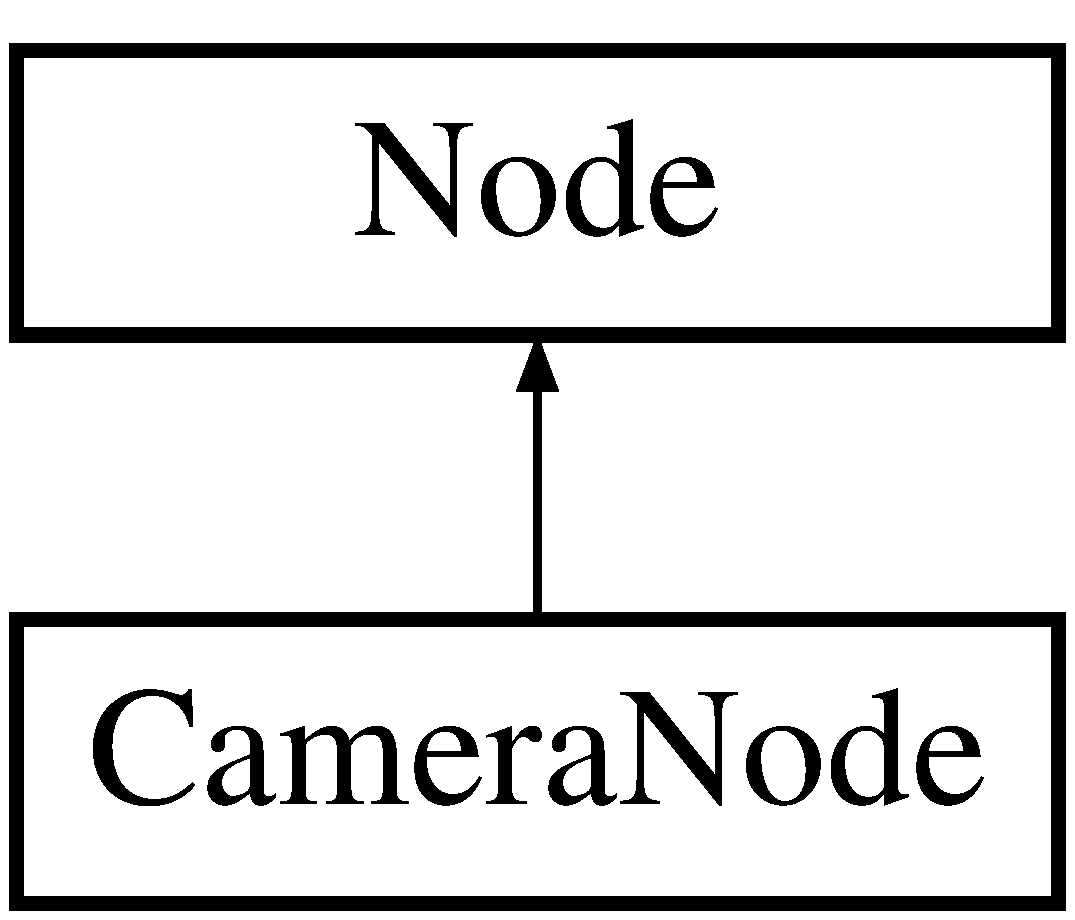
\includegraphics[height=2.000000cm]{classCameraNode}
\end{center}
\end{figure}
\subsection*{Public Member Functions}
\begin{DoxyCompactItemize}
\item 
\hypertarget{classCameraNode_a9975897c31197e56a4ea5bf7e0fb6f7a}{{\bfseries Camera\-Node} (const \hyperlink{classCamera}{Camera} \&c)}\label{classCameraNode_a9975897c31197e56a4ea5bf7e0fb6f7a}

\item 
void \hyperlink{classCameraNode_afc9b202cd080ee7e3a62e4e5676ab8a6}{execute} ()
\item 
void \hyperlink{classCameraNode_ad87fec242725e3eeb0546b8bfe8df6b7}{add\-Child} (const \hyperlink{classNode}{Node} $\ast$child)
\item 
void \hyperlink{classCameraNode_ae800e4fab63b5d3f9762a5532ffc201a}{camera\-Node\-Rotate} (const G\-Lfloat theta, const G\-Lfloat phi)
\item 
void \hyperlink{classCameraNode_adb8b1de4bcc623e2e4eebb4f4fd77e86}{camera\-Node\-Zoom} (const G\-Lfloat zoom)
\item 
void \hyperlink{classCameraNode_a994a0e7f079982f87d8470919fd3aea7}{camera\-Node\-Pan} (const G\-Lfloat pan\-X, const G\-Lfloat pan\-Y)
\end{DoxyCompactItemize}
\subsection*{Additional Inherited Members}


\subsection{Detailed Description}
Purpose\-: \hyperlink{classCameraNode}{Camera\-Node} wraps the camera class in a node object to add to the scene. \begin{DoxyAuthor}{Author}
Andrew Dang-\/\-Tran 
\end{DoxyAuthor}


\subsection{Member Function Documentation}
\hypertarget{classCameraNode_ad87fec242725e3eeb0546b8bfe8df6b7}{\index{Camera\-Node@{Camera\-Node}!add\-Child@{add\-Child}}
\index{add\-Child@{add\-Child}!CameraNode@{Camera\-Node}}
\subsubsection[{add\-Child}]{\setlength{\rightskip}{0pt plus 5cm}void Camera\-Node\-::add\-Child (
\begin{DoxyParamCaption}
\item[{const {\bf Node} $\ast$}]{child}
\end{DoxyParamCaption}
)}}\label{classCameraNode_ad87fec242725e3eeb0546b8bfe8df6b7}
\hyperlink{classCamera}{Camera} Nodes cannot have children, and this will throw an error \hypertarget{classCameraNode_a994a0e7f079982f87d8470919fd3aea7}{\index{Camera\-Node@{Camera\-Node}!camera\-Node\-Pan@{camera\-Node\-Pan}}
\index{camera\-Node\-Pan@{camera\-Node\-Pan}!CameraNode@{Camera\-Node}}
\subsubsection[{camera\-Node\-Pan}]{\setlength{\rightskip}{0pt plus 5cm}void Camera\-Node\-::camera\-Node\-Pan (
\begin{DoxyParamCaption}
\item[{const G\-Lfloat}]{pan\-X, }
\item[{const G\-Lfloat}]{pan\-Y}
\end{DoxyParamCaption}
)}}\label{classCameraNode_a994a0e7f079982f87d8470919fd3aea7}
Passes the values along to the camera to pan 
\begin{DoxyParams}{Parameters}
{\em pan\-X} & \\
\hline
{\em pan\-Y} & \\
\hline
\end{DoxyParams}
\hypertarget{classCameraNode_ae800e4fab63b5d3f9762a5532ffc201a}{\index{Camera\-Node@{Camera\-Node}!camera\-Node\-Rotate@{camera\-Node\-Rotate}}
\index{camera\-Node\-Rotate@{camera\-Node\-Rotate}!CameraNode@{Camera\-Node}}
\subsubsection[{camera\-Node\-Rotate}]{\setlength{\rightskip}{0pt plus 5cm}void Camera\-Node\-::camera\-Node\-Rotate (
\begin{DoxyParamCaption}
\item[{const G\-Lfloat}]{theta, }
\item[{const G\-Lfloat}]{phi}
\end{DoxyParamCaption}
)}}\label{classCameraNode_ae800e4fab63b5d3f9762a5532ffc201a}
Passes the values along to the camera to rotate 
\begin{DoxyParams}{Parameters}
{\em theta} & \\
\hline
{\em phi} & \\
\hline
\end{DoxyParams}
\hypertarget{classCameraNode_adb8b1de4bcc623e2e4eebb4f4fd77e86}{\index{Camera\-Node@{Camera\-Node}!camera\-Node\-Zoom@{camera\-Node\-Zoom}}
\index{camera\-Node\-Zoom@{camera\-Node\-Zoom}!CameraNode@{Camera\-Node}}
\subsubsection[{camera\-Node\-Zoom}]{\setlength{\rightskip}{0pt plus 5cm}void Camera\-Node\-::camera\-Node\-Zoom (
\begin{DoxyParamCaption}
\item[{const G\-Lfloat}]{zoom}
\end{DoxyParamCaption}
)}}\label{classCameraNode_adb8b1de4bcc623e2e4eebb4f4fd77e86}
Passes the values along to the camera to zoom 
\begin{DoxyParams}{Parameters}
{\em zoom} & \\
\hline
\end{DoxyParams}
\hypertarget{classCameraNode_afc9b202cd080ee7e3a62e4e5676ab8a6}{\index{Camera\-Node@{Camera\-Node}!execute@{execute}}
\index{execute@{execute}!CameraNode@{Camera\-Node}}
\subsubsection[{execute}]{\setlength{\rightskip}{0pt plus 5cm}void Camera\-Node\-::execute (
\begin{DoxyParamCaption}
{}
\end{DoxyParamCaption}
)\hspace{0.3cm}{\ttfamily [virtual]}}}\label{classCameraNode_afc9b202cd080ee7e3a62e4e5676ab8a6}
Sets the camera in the correct position 

Reimplemented from \hyperlink{classNode_a6890991303fcc6c9b2b3dec678c8b5db}{Node}.



The documentation for this class was generated from the following files\-:\begin{DoxyCompactItemize}
\item 
Camera\-Node.\-h\item 
Camera\-Node.\-c++\end{DoxyCompactItemize}

\hypertarget{classFace}{\section{Face Class Reference}
\label{classFace}\index{Face@{Face}}
}
\subsection*{Public Member Functions}
\begin{DoxyCompactItemize}
\item 
\hypertarget{classFace_a7655f5c584e03c266cba1cfbd6877e05}{{\bfseries Face} (const int $\ast$vertices)}\label{classFace_a7655f5c584e03c266cba1cfbd6877e05}

\item 
void \hyperlink{classFace_af200efb8cdd7ee66139bdf8be198c53e}{set\-Normal} (const G\-Lfloat $\ast$n)
\item 
void \hyperlink{classFace_a1486f1762166b2cc77b1806dfcc4a12a}{compute\-Center} (const vector$<$ \hyperlink{classVertex}{Vertex} $>$ \&vertices)
\item 
\hypertarget{classFace_a17212b0377c8279369d1b57bff5df503}{void {\bfseries draw\-Normal} () const }\label{classFace_a17212b0377c8279369d1b57bff5df503}

\item 
\hypertarget{classFace_a107b157049a2b38e12b4666babf62823}{G\-Lfloat $\ast$ {\bfseries get\-Normal} ()}\label{classFace_a107b157049a2b38e12b4666babf62823}

\item 
\hypertarget{classFace_a0e8c46dcca387d9dcdc0c4067cbea982}{int $\ast$ {\bfseries get\-Triangle\-Index} ()}\label{classFace_a0e8c46dcca387d9dcdc0c4067cbea982}

\end{DoxyCompactItemize}


\subsection{Member Function Documentation}
\hypertarget{classFace_a1486f1762166b2cc77b1806dfcc4a12a}{\index{Face@{Face}!compute\-Center@{compute\-Center}}
\index{compute\-Center@{compute\-Center}!Face@{Face}}
\subsubsection[{compute\-Center}]{\setlength{\rightskip}{0pt plus 5cm}void Face\-::compute\-Center (
\begin{DoxyParamCaption}
\item[{const vector$<$ {\bf Vertex} $>$ \&}]{vertices}
\end{DoxyParamCaption}
)}}\label{classFace_a1486f1762166b2cc77b1806dfcc4a12a}
Compute the center of the face to draw normal lines on 
\begin{DoxyParams}{Parameters}
{\em vertices} & -\/ the three vertices which make up the face \\
\hline
\end{DoxyParams}
\hypertarget{classFace_af200efb8cdd7ee66139bdf8be198c53e}{\index{Face@{Face}!set\-Normal@{set\-Normal}}
\index{set\-Normal@{set\-Normal}!Face@{Face}}
\subsubsection[{set\-Normal}]{\setlength{\rightskip}{0pt plus 5cm}void Face\-::set\-Normal (
\begin{DoxyParamCaption}
\item[{const G\-Lfloat $\ast$}]{n}
\end{DoxyParamCaption}
)}}\label{classFace_af200efb8cdd7ee66139bdf8be198c53e}
Compute the normal of the face 
\begin{DoxyParams}{Parameters}
{\em normal} & -\/ array of xyz\mbox{[}3\mbox{]} for the direction of the normal \\
\hline
\end{DoxyParams}


The documentation for this class was generated from the following files\-:\begin{DoxyCompactItemize}
\item 
Face.\-h\item 
Face.\-c++\end{DoxyCompactItemize}

\hypertarget{classGeomNode}{\section{Geom\-Node Class Reference}
\label{classGeomNode}\index{Geom\-Node@{Geom\-Node}}
}


{\ttfamily \#include $<$Geom\-Node.\-h$>$}

Inheritance diagram for Geom\-Node\-:\begin{figure}[H]
\begin{center}
\leavevmode
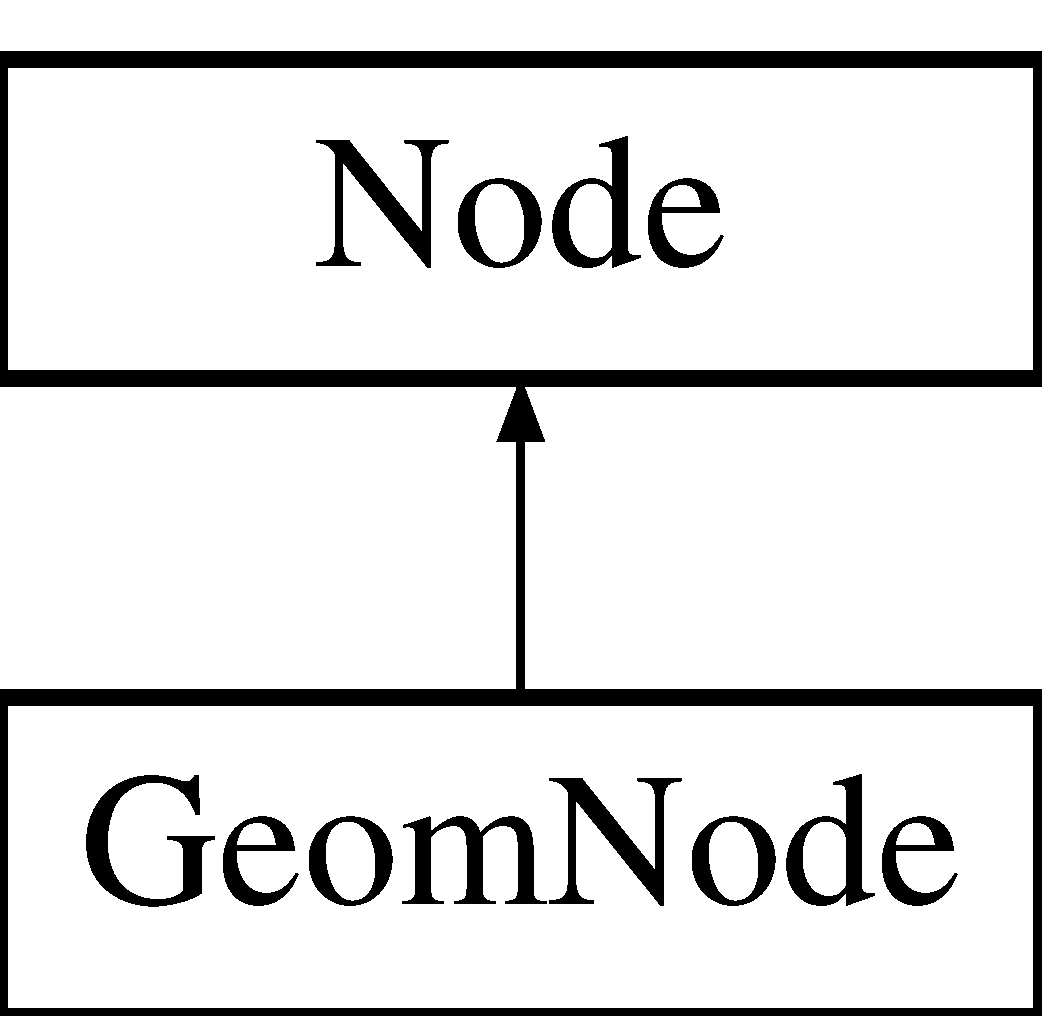
\includegraphics[height=2.000000cm]{classGeomNode}
\end{center}
\end{figure}
\subsection*{Public Member Functions}
\begin{DoxyCompactItemize}
\item 
\hypertarget{classGeomNode_a1474347796226f324cc7b1bc5a1eeae7}{{\bfseries Geom\-Node} (\hyperlink{classTrimeshLoader}{Trimesh\-Loader} \&loader, const string \&mesh\-Name, bool draw\-F\-N, bool draw\-V\-N, bool use\-F\-N)}\label{classGeomNode_a1474347796226f324cc7b1bc5a1eeae7}

\item 
void \hyperlink{classGeomNode_a9755aa5e3bbe2b746244405244064681}{execute} ()
\item 
\hypertarget{classGeomNode_af5bef5d3671dee78640b64109ed6de6c}{void {\bfseries set\-Parameters} (\hyperlink{classTrimeshLoader}{Trimesh\-Loader} \&loader, const string new\-Obj\-File, const bool draw\-F\-N, const bool draw\-V\-N, const bool use\-F\-N)}\label{classGeomNode_af5bef5d3671dee78640b64109ed6de6c}

\end{DoxyCompactItemize}
\subsection*{Additional Inherited Members}


\subsection{Detailed Description}
Purpose\-: Wraps the trimesh class in a node so it can be inserted in the scene. \begin{DoxyAuthor}{Author}
Andrew Dang-\/\-Tran 
\end{DoxyAuthor}


\subsection{Member Function Documentation}
\hypertarget{classGeomNode_a9755aa5e3bbe2b746244405244064681}{\index{Geom\-Node@{Geom\-Node}!execute@{execute}}
\index{execute@{execute}!GeomNode@{Geom\-Node}}
\subsubsection[{execute}]{\setlength{\rightskip}{0pt plus 5cm}void Geom\-Node\-::execute (
\begin{DoxyParamCaption}
{}
\end{DoxyParamCaption}
)\hspace{0.3cm}{\ttfamily [virtual]}}}\label{classGeomNode_a9755aa5e3bbe2b746244405244064681}
Renders the object and the face normals / vertex normals if necessary. 

Reimplemented from \hyperlink{classNode_a6890991303fcc6c9b2b3dec678c8b5db}{Node}.



The documentation for this class was generated from the following files\-:\begin{DoxyCompactItemize}
\item 
Geom\-Node.\-h\item 
Geom\-Node.\-c++\end{DoxyCompactItemize}

\hypertarget{classLight}{\section{Light Class Reference}
\label{classLight}\index{Light@{Light}}
}


{\ttfamily \#include $<$Light.\-h$>$}

\subsection*{Public Member Functions}
\begin{DoxyCompactItemize}
\item 
\hypertarget{classLight_a09bf6a8042fe3c716c8cfcad20a4756d}{{\bfseries Light} (const Light\-Type t, const G\-Lfloat $\ast$pos, const G\-Lfloat $\ast$sp\-D, const G\-Lfloat $\ast$a, const G\-Lfloat $\ast$d, const G\-Lfloat $\ast$s, const int l\-N)}\label{classLight_a09bf6a8042fe3c716c8cfcad20a4756d}

\item 
void \hyperlink{classLight_aeefdb2b26baca28698bddba8a6d4ec74}{set\-Light} ()
\item 
\hypertarget{classLight_a56b6d9d6e306a172d526f5d12a599db9}{void {\bfseries change\-Lighting} (const Light\-Type t, const G\-Lfloat $\ast$pos, const G\-Lfloat $\ast$sp\-D, const G\-Lfloat $\ast$a, const G\-Lfloat $\ast$d, const G\-Lfloat $\ast$s)}\label{classLight_a56b6d9d6e306a172d526f5d12a599db9}

\item 
\hypertarget{classLight_a61b430d820fb97d4d092407e93157aed}{void {\bfseries disable} () const }\label{classLight_a61b430d820fb97d4d092407e93157aed}

\end{DoxyCompactItemize}


\subsection{Detailed Description}
Encapsulates all of the variables of a typical Open\-G\-L light 

\subsection{Member Function Documentation}
\hypertarget{classLight_aeefdb2b26baca28698bddba8a6d4ec74}{\index{Light@{Light}!set\-Light@{set\-Light}}
\index{set\-Light@{set\-Light}!Light@{Light}}
\subsubsection[{set\-Light}]{\setlength{\rightskip}{0pt plus 5cm}void Light\-::set\-Light (
\begin{DoxyParamCaption}
{}
\end{DoxyParamCaption}
)}}\label{classLight_aeefdb2b26baca28698bddba8a6d4ec74}
Sets the light in the appropriate location and with the correct ambience, diffuse, and specular values. 

The documentation for this class was generated from the following files\-:\begin{DoxyCompactItemize}
\item 
Light.\-h\item 
Light.\-c++\end{DoxyCompactItemize}

\hypertarget{classLightNode}{\section{Light\-Node Class Reference}
\label{classLightNode}\index{Light\-Node@{Light\-Node}}
}


{\ttfamily \#include $<$Light\-Node.\-h$>$}

Inheritance diagram for Light\-Node\-:\begin{figure}[H]
\begin{center}
\leavevmode
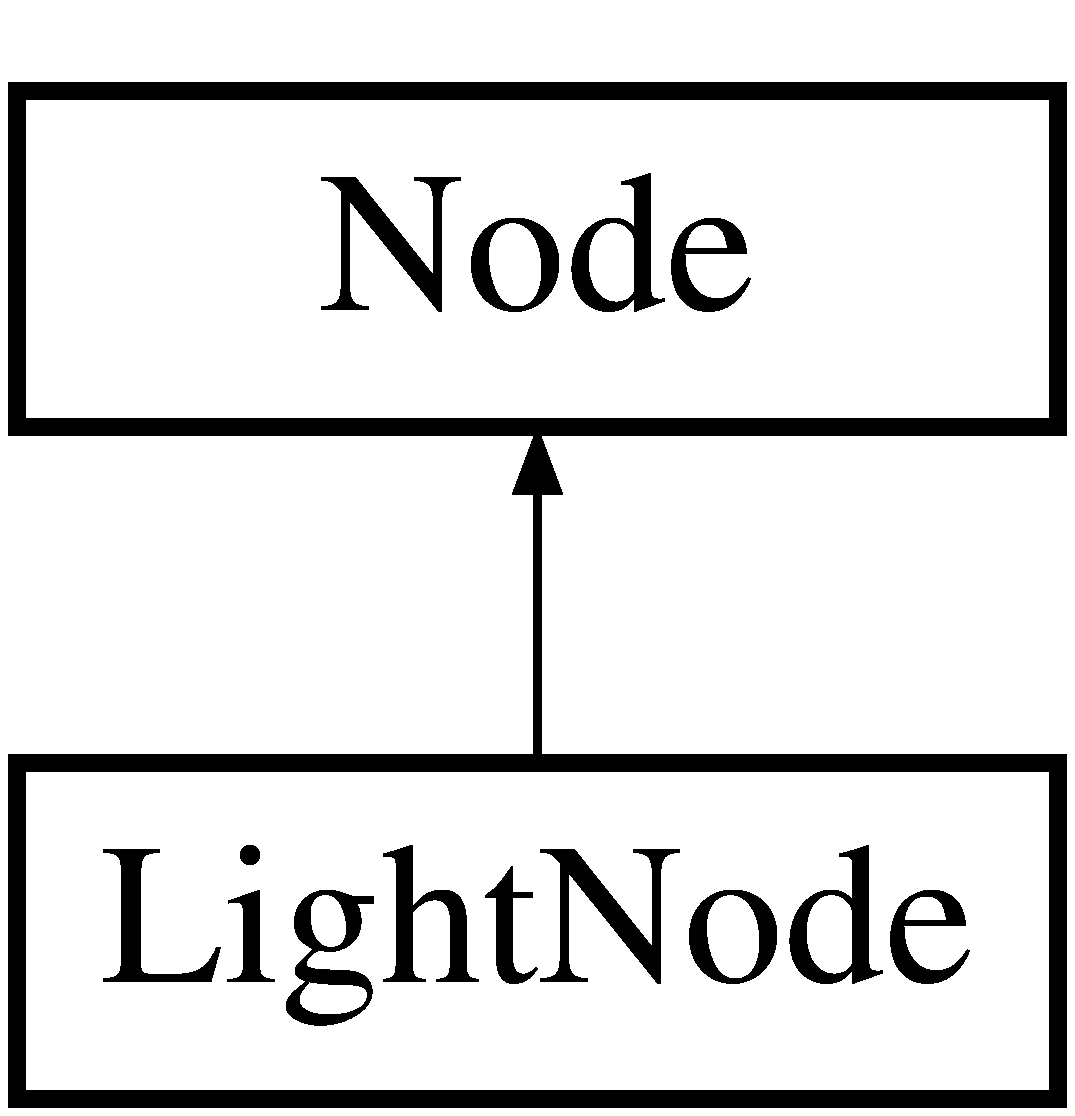
\includegraphics[height=2.000000cm]{classLightNode}
\end{center}
\end{figure}
\subsection*{Public Member Functions}
\begin{DoxyCompactItemize}
\item 
\hypertarget{classLightNode_af1c8654971c8c565770cbda60d0eb69c}{{\bfseries Light\-Node} (const \hyperlink{classLight}{Light} \&l)}\label{classLightNode_af1c8654971c8c565770cbda60d0eb69c}

\item 
void \hyperlink{classLightNode_ab75ed073b22f779c445a46741b40f3c7}{execute} ()
\item 
void \hyperlink{classLightNode_ad8e6562c22da8186eba945c775b80d67}{add\-Child} (const \hyperlink{classNode}{Node} $\ast$child)
\item 
\hypertarget{classLightNode_a9266a158c46c1ccb9ace10211cc9303d}{void {\bfseries set\-Parameters} (const Light\-Type t, const G\-Lfloat $\ast$pos, const G\-Lfloat $\ast$sp\-D, const G\-Lfloat $\ast$a, const G\-Lfloat $\ast$d, const G\-Lfloat $\ast$s)}\label{classLightNode_a9266a158c46c1ccb9ace10211cc9303d}

\item 
\hypertarget{classLightNode_a57ad0c3f24fdaa0543541055c9c753f4}{void {\bfseries disable\-Light} () const }\label{classLightNode_a57ad0c3f24fdaa0543541055c9c753f4}

\end{DoxyCompactItemize}
\subsection*{Additional Inherited Members}


\subsection{Detailed Description}
Purpose\-: wraps the light class in a node which can be entered in the scene. \begin{DoxyAuthor}{Author}
Andrew Dang-\/\-Tran 
\end{DoxyAuthor}


\subsection{Member Function Documentation}
\hypertarget{classLightNode_ad8e6562c22da8186eba945c775b80d67}{\index{Light\-Node@{Light\-Node}!add\-Child@{add\-Child}}
\index{add\-Child@{add\-Child}!LightNode@{Light\-Node}}
\subsubsection[{add\-Child}]{\setlength{\rightskip}{0pt plus 5cm}void Light\-Node\-::add\-Child (
\begin{DoxyParamCaption}
\item[{const {\bf Node} $\ast$}]{child}
\end{DoxyParamCaption}
)}}\label{classLightNode_ad8e6562c22da8186eba945c775b80d67}
\hyperlink{classLight}{Light} Nodes cannot have children, and this will throw an error A simple string with an error message is thrown. \hypertarget{classLightNode_ab75ed073b22f779c445a46741b40f3c7}{\index{Light\-Node@{Light\-Node}!execute@{execute}}
\index{execute@{execute}!LightNode@{Light\-Node}}
\subsubsection[{execute}]{\setlength{\rightskip}{0pt plus 5cm}void Light\-Node\-::execute (
\begin{DoxyParamCaption}
{}
\end{DoxyParamCaption}
)\hspace{0.3cm}{\ttfamily [virtual]}}}\label{classLightNode_ab75ed073b22f779c445a46741b40f3c7}
Sets the light in right position with parameters given. 

Reimplemented from \hyperlink{classNode_a6890991303fcc6c9b2b3dec678c8b5db}{Node}.



The documentation for this class was generated from the following files\-:\begin{DoxyCompactItemize}
\item 
Light\-Node.\-h\item 
Light\-Node.\-c++\end{DoxyCompactItemize}

\hypertarget{classNode}{\section{Node Class Reference}
\label{classNode}\index{Node@{Node}}
}


{\ttfamily \#include $<$Node.\-h$>$}

Inheritance diagram for Node\-:\begin{figure}[H]
\begin{center}
\leavevmode
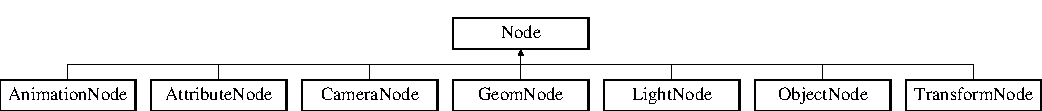
\includegraphics[height=1.495327cm]{classNode}
\end{center}
\end{figure}
\subsection*{Public Member Functions}
\begin{DoxyCompactItemize}
\item 
virtual void \hyperlink{classNode_a6890991303fcc6c9b2b3dec678c8b5db}{execute} ()
\item 
\hypertarget{classNode_ae17dff73e3a5026946eaf24920454e9d}{const int {\bfseries get\-I\-D} () const }\label{classNode_ae17dff73e3a5026946eaf24920454e9d}

\item 
\hypertarget{classNode_a599186538d9354a563ea7175ed85ca4b}{const vector$<$ \hyperlink{classNode}{Node} $\ast$ $>$ \& {\bfseries get\-Children} () const }\label{classNode_a599186538d9354a563ea7175ed85ca4b}

\item 
\hypertarget{classNode_a132699398b350e83b548a5645e69beb0}{void {\bfseries add\-Child} (\hyperlink{classNode}{Node} $\ast$child)}\label{classNode_a132699398b350e83b548a5645e69beb0}

\item 
void \hyperlink{classNode_ad0665d6541266c8bdbdc3169674cb6ae}{traverse\-Children} ()
\item 
\hypertarget{classNode_a1f2cee9006b507c74d4c0efc2a0f0b19}{const \hyperlink{classNode}{Node} $\ast$ {\bfseries get\-Parent} () const }\label{classNode_a1f2cee9006b507c74d4c0efc2a0f0b19}

\item 
\hypertarget{classNode_a220a8d64cb0df1cce083ed38c1260615}{\hyperlink{classNode}{Node} $\ast$ {\bfseries get\-Parent} ()}\label{classNode_a220a8d64cb0df1cce083ed38c1260615}

\item 
\hypertarget{classNode_a06dbfc5f19f4e527619e2bd99881bd91}{const Node\-Type {\bfseries get\-Type} () const }\label{classNode_a06dbfc5f19f4e527619e2bd99881bd91}

\item 
\hypertarget{classNode_a3a2abb80f0a1b618161615353e889d3e}{void {\bfseries remove\-Child} (\hyperlink{classNode}{Node} $\ast$target\-Child)}\label{classNode_a3a2abb80f0a1b618161615353e889d3e}

\end{DoxyCompactItemize}
\subsection*{Protected Attributes}
\begin{DoxyCompactItemize}
\item 
\hypertarget{classNode_ad8184598cdea70e4bbdfd76f2b0f9e85}{\hyperlink{classNode}{Node} $\ast$ {\bfseries parent}}\label{classNode_ad8184598cdea70e4bbdfd76f2b0f9e85}

\item 
\hypertarget{classNode_a24d3a13419098b7ce6f1a760286f66e3}{Node\-Type {\bfseries type}}\label{classNode_a24d3a13419098b7ce6f1a760286f66e3}

\end{DoxyCompactItemize}


\subsection{Detailed Description}
Base node class with typical n-\/tree parent child relations. 

\subsection{Member Function Documentation}
\hypertarget{classNode_a6890991303fcc6c9b2b3dec678c8b5db}{\index{Node@{Node}!execute@{execute}}
\index{execute@{execute}!Node@{Node}}
\subsubsection[{execute}]{\setlength{\rightskip}{0pt plus 5cm}void Node\-::execute (
\begin{DoxyParamCaption}
{}
\end{DoxyParamCaption}
)\hspace{0.3cm}{\ttfamily [virtual]}}}\label{classNode_a6890991303fcc6c9b2b3dec678c8b5db}
Do the determined action for each node. 

Reimplemented in \hyperlink{classAttributeNode_ad6fb6f07dc9728e066c769c35c321f25}{Attribute\-Node}, \hyperlink{classAnimationNode_a0b0bb275a3f89f45aedd35f41f459f9f}{Animation\-Node}, \hyperlink{classGeomNode_a9755aa5e3bbe2b746244405244064681}{Geom\-Node}, \hyperlink{classObjectNode_ab354580ede8a53ea2986b9a5251849fa}{Object\-Node}, \hyperlink{classCameraNode_afc9b202cd080ee7e3a62e4e5676ab8a6}{Camera\-Node}, \hyperlink{classLightNode_ab75ed073b22f779c445a46741b40f3c7}{Light\-Node}, and \hyperlink{classTransformNode_a746be4bb9fd24686ff2a6ad49c08c986}{Transform\-Node}.

\hypertarget{classNode_ad0665d6541266c8bdbdc3169674cb6ae}{\index{Node@{Node}!traverse\-Children@{traverse\-Children}}
\index{traverse\-Children@{traverse\-Children}!Node@{Node}}
\subsubsection[{traverse\-Children}]{\setlength{\rightskip}{0pt plus 5cm}void Node\-::traverse\-Children (
\begin{DoxyParamCaption}
{}
\end{DoxyParamCaption}
)}}\label{classNode_ad0665d6541266c8bdbdc3169674cb6ae}
Traverses through the scene graph starting from the calling node. Calls execute on each node it passes. Makes sure to push and pop the correct matrixes so not everything is effected by every transform. 

The documentation for this class was generated from the following files\-:\begin{DoxyCompactItemize}
\item 
Node.\-h\item 
Node.\-c++\end{DoxyCompactItemize}

\hypertarget{classObjectNode}{\section{Object\-Node Class Reference}
\label{classObjectNode}\index{Object\-Node@{Object\-Node}}
}


{\ttfamily \#include $<$Object\-Node.\-h$>$}

Inheritance diagram for Object\-Node\-:\begin{figure}[H]
\begin{center}
\leavevmode
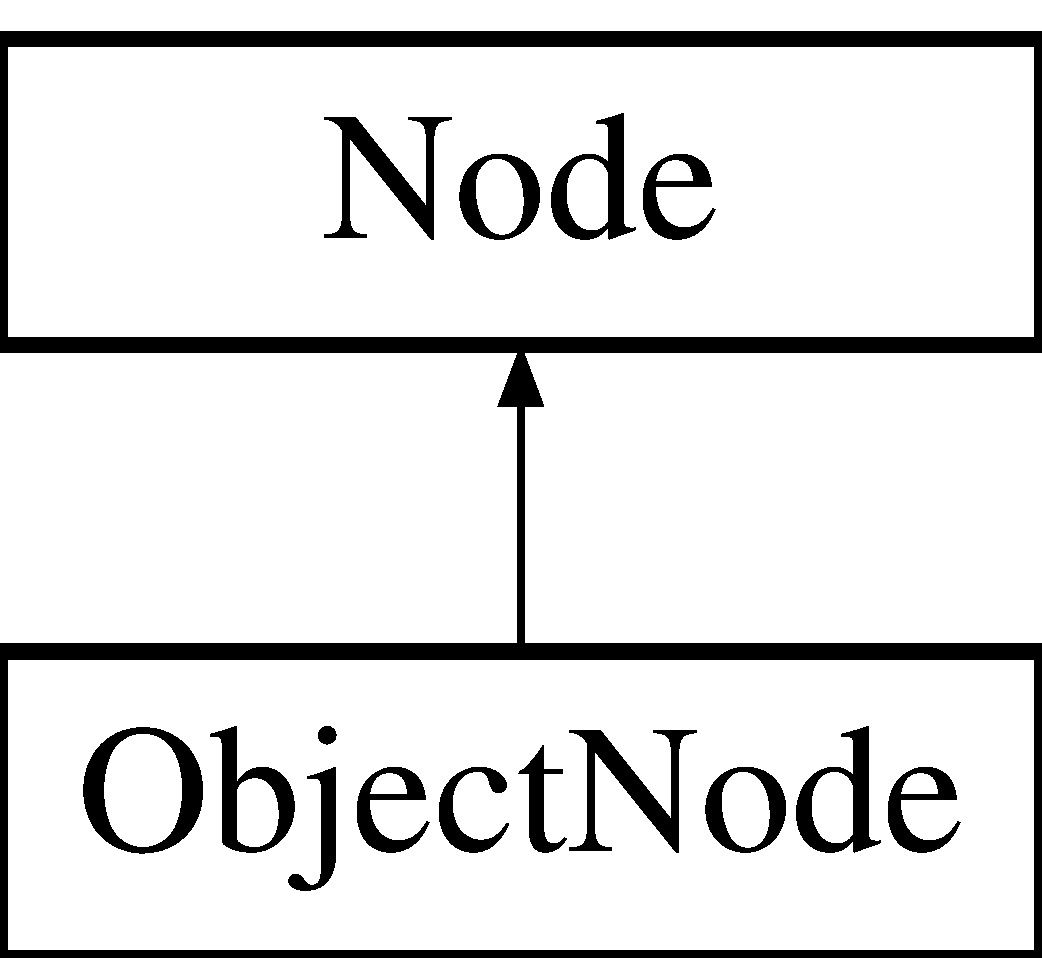
\includegraphics[height=2.000000cm]{classObjectNode}
\end{center}
\end{figure}
\subsection*{Public Member Functions}
\begin{DoxyCompactItemize}
\item 
\hypertarget{classObjectNode_aa63236a1b5905933b88383383e7f1964}{{\bfseries Object\-Node} (const string \&n=string(\char`\"{}World\char`\"{}))}\label{classObjectNode_aa63236a1b5905933b88383383e7f1964}

\item 
\hypertarget{classObjectNode_a3743ff7e3b278d3498bf2db020bcfd32}{const string {\bfseries get\-Name} ()}\label{classObjectNode_a3743ff7e3b278d3498bf2db020bcfd32}

\item 
void \hyperlink{classObjectNode_ab354580ede8a53ea2986b9a5251849fa}{execute} ()
\item 
\hypertarget{classObjectNode_a478bf4eb8026b01fcafa73e5346ceed8}{void {\bfseries set\-Name} (const string new\-Name)}\label{classObjectNode_a478bf4eb8026b01fcafa73e5346ceed8}

\end{DoxyCompactItemize}
\subsection*{Additional Inherited Members}


\subsection{Detailed Description}
Purpose\-: Class stores face/vertex information \begin{DoxyAuthor}{Author}
Andrew Dang-\/\-Tran Object\-Nodes serve as a link between other objects, and groups them together with a name. 
\end{DoxyAuthor}


\subsection{Member Function Documentation}
\hypertarget{classObjectNode_ab354580ede8a53ea2986b9a5251849fa}{\index{Object\-Node@{Object\-Node}!execute@{execute}}
\index{execute@{execute}!ObjectNode@{Object\-Node}}
\subsubsection[{execute}]{\setlength{\rightskip}{0pt plus 5cm}void Object\-Node\-::execute (
\begin{DoxyParamCaption}
{}
\end{DoxyParamCaption}
)\hspace{0.3cm}{\ttfamily [virtual]}}}\label{classObjectNode_ab354580ede8a53ea2986b9a5251849fa}
Doesn't do anything for Object\-Nodes. 

Reimplemented from \hyperlink{classNode_a6890991303fcc6c9b2b3dec678c8b5db}{Node}.



The documentation for this class was generated from the following files\-:\begin{DoxyCompactItemize}
\item 
Object\-Node.\-h\item 
Object\-Node.\-c++\end{DoxyCompactItemize}

\hypertarget{classSceneGraph}{\section{Scene\-Graph Class Reference}
\label{classSceneGraph}\index{Scene\-Graph@{Scene\-Graph}}
}


{\ttfamily \#include $<$Scene\-Graph.\-h$>$}

\subsection*{Public Member Functions}
\begin{DoxyCompactItemize}
\item 
\hyperlink{classSceneGraph_a10cb00465716a38ceff196f9ee220620}{Scene\-Graph} ()
\item 
\hyperlink{classSceneGraph_a4f7164675d0787d1ab73dea9da097db7}{$\sim$\-Scene\-Graph} ()
\item 
void \hyperlink{classSceneGraph_aec1ab0dea305ce38e77fdf0c2eff663a}{traversal} ()
\item 
bool \hyperlink{classSceneGraph_a6b81c95f19b42385e5f0c97212884bb7}{add\-Object\-Node} (const int parent\-I\-D, string n)
\item 
void \hyperlink{classSceneGraph_aa700695f92cfc45d639f12013c5d8041}{edit\-Object\-Node} (const int node\-I\-D, const string new\-Name)
\item 
bool \hyperlink{classSceneGraph_a485de4aab6468a0b744c90e6300b4560}{add\-Geom\-Node} (const int parent\-I\-D, string \&file\-Name, const bool draw\-F\-N, const bool draw\-V\-N, const bool use\-F\-N)
\item 
void \hyperlink{classSceneGraph_a4d3d9842a52c7d08a7ec8167e7b63f22}{edit\-Geom\-Node} (const int node\-I\-D, string \&new\-File\-Name, const bool draw\-F\-N, const bool draw\-V\-N, const bool use\-F\-N)
\item 
bool \hyperlink{classSceneGraph_aa08d1e21cd6eb46623aedf5365515476}{add\-Transform\-Node} (const int parent\-I\-D, const Transform\-Type type, const G\-Lfloat $\ast$args)
\item 
void \hyperlink{classSceneGraph_a0ee6318b0f71b81fc70587038aa06fcd}{edit\-Transform\-Node} (const int node\-I\-D, const Transform\-Type t, const G\-Lfloat $\ast$new\-Args)
\item 
bool \hyperlink{classSceneGraph_a50057912223b1fde361a661846efc30a}{add\-Animation\-Node} (const int parent\-I\-D, const Transform\-Type type, const G\-Lfloat $\ast$args, float cycle\-Time)
\item 
void \hyperlink{classSceneGraph_a3926097010b35104826c42d3e880eaf1}{edit\-Animation\-Node} (const int node\-I\-D, const Transform\-Type t, const G\-Lfloat $\ast$new\-Args, float new\-Cycle\-Time)
\item 
bool \hyperlink{classSceneGraph_a08c22573bfb236c5d100d2e0852eb827}{add\-Attribute\-Node} (const int parent\-I\-D, const Mode mode)
\item 
void \hyperlink{classSceneGraph_a2b54cadc617d3cdc828005ece998e3d0}{edit\-Attribute\-Node} (const int node\-I\-D, const Mode new\-Mode)
\item 
bool \hyperlink{classSceneGraph_aa5ce83892a3786d9a6ff6a05994d1323}{add\-Light\-Node} (const int parent\-I\-D, Light\-Type type, const G\-Lfloat $\ast$position, const G\-Lfloat $\ast$spot\-Direction, const G\-Lfloat $\ast$ambient, const G\-Lfloat $\ast$diffuse, const G\-Lfloat $\ast$specular)
\item 
void \hyperlink{classSceneGraph_ae7eaaa12346ede54a8a6ce4c6bf5d89d}{edit\-Light\-Node} (const int node\-I\-D, Light\-Type new\-Type, const G\-Lfloat $\ast$new\-Pos, const G\-Lfloat $\ast$new\-Spot\-D, const G\-Lfloat $\ast$new\-Amb, const G\-Lfloat $\ast$new\-Dif, const G\-Lfloat $\ast$new\-Spec)
\item 
bool \hyperlink{classSceneGraph_a5d945279fb8acf87519ec0050486441c}{delete\-Node} (const int id)
\item 
void \hyperlink{classSceneGraph_addbd59946f266cd0f29bc47e68918a0a}{camera\-Rotate} (const G\-Lfloat theta, const G\-Lfloat phi)
\item 
void \hyperlink{classSceneGraph_a595a0a4fb507ce008bca05ccf284c5ab}{camera\-Zoom} (const G\-Lfloat zoom)
\item 
void \hyperlink{classSceneGraph_a8fad2a82153647e4a91a197f2445a7ca}{camera\-Pan} (const G\-Lfloat pan\-X, const G\-Lfloat pan\-Y)
\item 
\hypertarget{classSceneGraph_a3c26e0dda954dd444ade94c18bf831e8}{Node\-Type {\bfseries get\-Node\-Type} (const int id)}\label{classSceneGraph_a3c26e0dda954dd444ade94c18bf831e8}

\end{DoxyCompactItemize}


\subsection{Detailed Description}
Purpose\-: Class which brings all the nodes together, and creates the scene. \begin{DoxyAuthor}{Author}
Andrew Dang-\/\-Tran 
\end{DoxyAuthor}


\subsection{Constructor \& Destructor Documentation}
\hypertarget{classSceneGraph_a10cb00465716a38ceff196f9ee220620}{\index{Scene\-Graph@{Scene\-Graph}!Scene\-Graph@{Scene\-Graph}}
\index{Scene\-Graph@{Scene\-Graph}!SceneGraph@{Scene\-Graph}}
\subsubsection[{Scene\-Graph}]{\setlength{\rightskip}{0pt plus 5cm}Scene\-Graph\-::\-Scene\-Graph (
\begin{DoxyParamCaption}
{}
\end{DoxyParamCaption}
)}}\label{classSceneGraph_a10cb00465716a38ceff196f9ee220620}
Construct a typical \hyperlink{classSceneGraph}{Scene\-Graph} with a root \char`\"{}\-World\char`\"{} node, (I\-D = 0) \hyperlink{classCamera}{Camera} \hyperlink{classNode}{Node} (I\-D = 1) and \hyperlink{classLight}{Light} \hyperlink{classNode}{Node} (I\-D = 2) The nodes your adding should be the children of the root. \hypertarget{classSceneGraph_a4f7164675d0787d1ab73dea9da097db7}{\index{Scene\-Graph@{Scene\-Graph}!$\sim$\-Scene\-Graph@{$\sim$\-Scene\-Graph}}
\index{$\sim$\-Scene\-Graph@{$\sim$\-Scene\-Graph}!SceneGraph@{Scene\-Graph}}
\subsubsection[{$\sim$\-Scene\-Graph}]{\setlength{\rightskip}{0pt plus 5cm}Scene\-Graph\-::$\sim$\-Scene\-Graph (
\begin{DoxyParamCaption}
{}
\end{DoxyParamCaption}
)}}\label{classSceneGraph_a4f7164675d0787d1ab73dea9da097db7}
Makes sure to properly free the memory of all the Nodes in the Scene Graph 

\subsection{Member Function Documentation}
\hypertarget{classSceneGraph_a50057912223b1fde361a661846efc30a}{\index{Scene\-Graph@{Scene\-Graph}!add\-Animation\-Node@{add\-Animation\-Node}}
\index{add\-Animation\-Node@{add\-Animation\-Node}!SceneGraph@{Scene\-Graph}}
\subsubsection[{add\-Animation\-Node}]{\setlength{\rightskip}{0pt plus 5cm}bool Scene\-Graph\-::add\-Animation\-Node (
\begin{DoxyParamCaption}
\item[{const int}]{parent\-I\-D, }
\item[{const Transform\-Type}]{type, }
\item[{const G\-Lfloat $\ast$}]{args, }
\item[{float}]{cycle\-Time}
\end{DoxyParamCaption}
)}}\label{classSceneGraph_a50057912223b1fde361a661846efc30a}
Add an Animation \hyperlink{classNode}{Node} to the Scene Graph 
\begin{DoxyParams}{Parameters}
{\em parent\-I\-D} & \\
\hline
{\em Transform\-Type} & -\/ Translate, Scale, Rotate \\
\hline
{\em Arguments} & -\/ x y z Theta array \\
\hline
{\em cycle\-Time} & -\/ Estimate of Seconds \\
\hline
\end{DoxyParams}
\hypertarget{classSceneGraph_a08c22573bfb236c5d100d2e0852eb827}{\index{Scene\-Graph@{Scene\-Graph}!add\-Attribute\-Node@{add\-Attribute\-Node}}
\index{add\-Attribute\-Node@{add\-Attribute\-Node}!SceneGraph@{Scene\-Graph}}
\subsubsection[{add\-Attribute\-Node}]{\setlength{\rightskip}{0pt plus 5cm}bool Scene\-Graph\-::add\-Attribute\-Node (
\begin{DoxyParamCaption}
\item[{const int}]{parent\-I\-D, }
\item[{const Mode}]{mode}
\end{DoxyParamCaption}
)}}\label{classSceneGraph_a08c22573bfb236c5d100d2e0852eb827}
Add an \hyperlink{classAnimationNode}{Animation\-Node} to the Scene Graph 
\begin{DoxyParams}{Parameters}
{\em parent\-I\-D} & \\
\hline
{\em Mode} & -\/ P\-O\-I\-N\-T\-\_\-\-M\-O\-D\-E, W\-I\-R\-E\-F\-R\-A\-M\-E\-\_\-\-M\-O\-D\-E, S\-O\-L\-I\-D\-\_\-\-M\-O\-D\-E, S\-H\-A\-D\-E\-D\-\_\-\-M\-O\-D\-E \\
\hline
\end{DoxyParams}
\hypertarget{classSceneGraph_a485de4aab6468a0b744c90e6300b4560}{\index{Scene\-Graph@{Scene\-Graph}!add\-Geom\-Node@{add\-Geom\-Node}}
\index{add\-Geom\-Node@{add\-Geom\-Node}!SceneGraph@{Scene\-Graph}}
\subsubsection[{add\-Geom\-Node}]{\setlength{\rightskip}{0pt plus 5cm}bool Scene\-Graph\-::add\-Geom\-Node (
\begin{DoxyParamCaption}
\item[{const int}]{parent\-I\-D, }
\item[{string \&}]{file\-Name, }
\item[{const bool}]{draw\-F\-N, }
\item[{const bool}]{draw\-V\-N, }
\item[{const bool}]{use\-F\-N}
\end{DoxyParamCaption}
)}}\label{classSceneGraph_a485de4aab6468a0b744c90e6300b4560}
Add a Geometry \hyperlink{classNode}{Node} to the Scene Graph 
\begin{DoxyParams}{Parameters}
{\em parent\-I\-D} & \\
\hline
{\em draw\-Face\-Normals} & -\/ show the lines which represent face normals \\
\hline
{\em draw\-Vertex\-Normals} & -\/ show the lines representing vertex normals \\
\hline
{\em use\-Face\-Normals} & -\/ use face or vertex normals for shading \\
\hline
\end{DoxyParams}
\hypertarget{classSceneGraph_aa5ce83892a3786d9a6ff6a05994d1323}{\index{Scene\-Graph@{Scene\-Graph}!add\-Light\-Node@{add\-Light\-Node}}
\index{add\-Light\-Node@{add\-Light\-Node}!SceneGraph@{Scene\-Graph}}
\subsubsection[{add\-Light\-Node}]{\setlength{\rightskip}{0pt plus 5cm}bool Scene\-Graph\-::add\-Light\-Node (
\begin{DoxyParamCaption}
\item[{const int}]{parent\-I\-D, }
\item[{Light\-Type}]{type, }
\item[{const G\-Lfloat $\ast$}]{position, }
\item[{const G\-Lfloat $\ast$}]{spot\-Direction, }
\item[{const G\-Lfloat $\ast$}]{ambient, }
\item[{const G\-Lfloat $\ast$}]{diffuse, }
\item[{const G\-Lfloat $\ast$}]{specular}
\end{DoxyParamCaption}
)}}\label{classSceneGraph_aa5ce83892a3786d9a6ff6a05994d1323}
Add a \hyperlink{classLight}{Light} \hyperlink{classNode}{Node} to the Scene Graph 
\begin{DoxyParams}{Parameters}
{\em parent\-I\-D} & \\
\hline
{\em Light\-Type} & -\/ P\-O\-I\-N\-T, D\-I\-R\-E\-C\-T\-I\-O\-N\-A\-L \\
\hline
{\em position} & -\/ x y z array \\
\hline
{\em spot\-Direction} & -\/ x y z array \\
\hline
{\em ambient} & -\/ r g b i array \\
\hline
{\em diffuse} & -\/ r g b i array \\
\hline
{\em specular} & -\/ r g b i array \\
\hline
\end{DoxyParams}
\hypertarget{classSceneGraph_a6b81c95f19b42385e5f0c97212884bb7}{\index{Scene\-Graph@{Scene\-Graph}!add\-Object\-Node@{add\-Object\-Node}}
\index{add\-Object\-Node@{add\-Object\-Node}!SceneGraph@{Scene\-Graph}}
\subsubsection[{add\-Object\-Node}]{\setlength{\rightskip}{0pt plus 5cm}bool Scene\-Graph\-::add\-Object\-Node (
\begin{DoxyParamCaption}
\item[{const int}]{parent\-I\-D, }
\item[{string}]{n}
\end{DoxyParamCaption}
)}}\label{classSceneGraph_a6b81c95f19b42385e5f0c97212884bb7}
Add an \hyperlink{classObjectNode}{Object\-Node} to the Scene Graph 
\begin{DoxyParams}{Parameters}
{\em parent\-I\-D} & \\
\hline
{\em name} & \\
\hline
\end{DoxyParams}
\hypertarget{classSceneGraph_aa08d1e21cd6eb46623aedf5365515476}{\index{Scene\-Graph@{Scene\-Graph}!add\-Transform\-Node@{add\-Transform\-Node}}
\index{add\-Transform\-Node@{add\-Transform\-Node}!SceneGraph@{Scene\-Graph}}
\subsubsection[{add\-Transform\-Node}]{\setlength{\rightskip}{0pt plus 5cm}bool Scene\-Graph\-::add\-Transform\-Node (
\begin{DoxyParamCaption}
\item[{const int}]{parent\-I\-D, }
\item[{const Transform\-Type}]{type, }
\item[{const G\-Lfloat $\ast$}]{args}
\end{DoxyParamCaption}
)}}\label{classSceneGraph_aa08d1e21cd6eb46623aedf5365515476}
Add a \hyperlink{classTransform}{Transform} \hyperlink{classNode}{Node} to the Scene Graph 
\begin{DoxyParams}{Parameters}
{\em parent\-I\-D} & \\
\hline
{\em Transform\-Type} & -\/ Translate, Scale, Rotate \\
\hline
{\em Arguments} & -\/ x y z Theta array \\
\hline
\end{DoxyParams}
\hypertarget{classSceneGraph_a8fad2a82153647e4a91a197f2445a7ca}{\index{Scene\-Graph@{Scene\-Graph}!camera\-Pan@{camera\-Pan}}
\index{camera\-Pan@{camera\-Pan}!SceneGraph@{Scene\-Graph}}
\subsubsection[{camera\-Pan}]{\setlength{\rightskip}{0pt plus 5cm}void Scene\-Graph\-::camera\-Pan (
\begin{DoxyParamCaption}
\item[{const G\-Lfloat}]{pan\-X, }
\item[{const G\-Lfloat}]{pan\-Y}
\end{DoxyParamCaption}
)}}\label{classSceneGraph_a8fad2a82153647e4a91a197f2445a7ca}
pan the camera 
\begin{DoxyParams}{Parameters}
{\em pan\-X} & \\
\hline
{\em pan\-Y} & \\
\hline
\end{DoxyParams}
\hypertarget{classSceneGraph_addbd59946f266cd0f29bc47e68918a0a}{\index{Scene\-Graph@{Scene\-Graph}!camera\-Rotate@{camera\-Rotate}}
\index{camera\-Rotate@{camera\-Rotate}!SceneGraph@{Scene\-Graph}}
\subsubsection[{camera\-Rotate}]{\setlength{\rightskip}{0pt plus 5cm}void Scene\-Graph\-::camera\-Rotate (
\begin{DoxyParamCaption}
\item[{const G\-Lfloat}]{theta, }
\item[{const G\-Lfloat}]{phi}
\end{DoxyParamCaption}
)}}\label{classSceneGraph_addbd59946f266cd0f29bc47e68918a0a}
rotate the camera 
\begin{DoxyParams}{Parameters}
{\em theta} & \\
\hline
{\em phi} & \\
\hline
\end{DoxyParams}
\hypertarget{classSceneGraph_a595a0a4fb507ce008bca05ccf284c5ab}{\index{Scene\-Graph@{Scene\-Graph}!camera\-Zoom@{camera\-Zoom}}
\index{camera\-Zoom@{camera\-Zoom}!SceneGraph@{Scene\-Graph}}
\subsubsection[{camera\-Zoom}]{\setlength{\rightskip}{0pt plus 5cm}void Scene\-Graph\-::camera\-Zoom (
\begin{DoxyParamCaption}
\item[{const G\-Lfloat}]{zoom}
\end{DoxyParamCaption}
)}}\label{classSceneGraph_a595a0a4fb507ce008bca05ccf284c5ab}
zoom the camera 
\begin{DoxyParams}{Parameters}
{\em zoom} & \\
\hline
\end{DoxyParams}
\hypertarget{classSceneGraph_a5d945279fb8acf87519ec0050486441c}{\index{Scene\-Graph@{Scene\-Graph}!delete\-Node@{delete\-Node}}
\index{delete\-Node@{delete\-Node}!SceneGraph@{Scene\-Graph}}
\subsubsection[{delete\-Node}]{\setlength{\rightskip}{0pt plus 5cm}bool Scene\-Graph\-::delete\-Node (
\begin{DoxyParamCaption}
\item[{const int}]{id}
\end{DoxyParamCaption}
)}}\label{classSceneGraph_a5d945279fb8acf87519ec0050486441c}
Delete a node and all of its children 
\begin{DoxyParams}{Parameters}
{\em id} & \\
\hline
\end{DoxyParams}
May need to change this to make these nodes children have their grandparent as $\ast$ parent\hypertarget{classSceneGraph_a3926097010b35104826c42d3e880eaf1}{\index{Scene\-Graph@{Scene\-Graph}!edit\-Animation\-Node@{edit\-Animation\-Node}}
\index{edit\-Animation\-Node@{edit\-Animation\-Node}!SceneGraph@{Scene\-Graph}}
\subsubsection[{edit\-Animation\-Node}]{\setlength{\rightskip}{0pt plus 5cm}void Scene\-Graph\-::edit\-Animation\-Node (
\begin{DoxyParamCaption}
\item[{const int}]{node\-I\-D, }
\item[{const Transform\-Type}]{t, }
\item[{const G\-Lfloat $\ast$}]{new\-Args, }
\item[{float}]{new\-Cycle\-Time}
\end{DoxyParamCaption}
)}}\label{classSceneGraph_a3926097010b35104826c42d3e880eaf1}
Edit an \hyperlink{classAnimationNode}{Animation\-Node} within the Scene Graph 
\begin{DoxyParams}{Parameters}
{\em node\-I\-D} & \\
\hline
{\em new\-Transform\-Type} & -\/ Translate, Scale, Rotate \\
\hline
{\em new\-Arguments} & -\/ x y z Theta array \\
\hline
{\em newcycle\-Time} & -\/ Estimate of Seconds for the animation complete and restart. \\
\hline
\end{DoxyParams}
\hypertarget{classSceneGraph_a2b54cadc617d3cdc828005ece998e3d0}{\index{Scene\-Graph@{Scene\-Graph}!edit\-Attribute\-Node@{edit\-Attribute\-Node}}
\index{edit\-Attribute\-Node@{edit\-Attribute\-Node}!SceneGraph@{Scene\-Graph}}
\subsubsection[{edit\-Attribute\-Node}]{\setlength{\rightskip}{0pt plus 5cm}void Scene\-Graph\-::edit\-Attribute\-Node (
\begin{DoxyParamCaption}
\item[{const int}]{node\-I\-D, }
\item[{const Mode}]{new\-Mode}
\end{DoxyParamCaption}
)}}\label{classSceneGraph_a2b54cadc617d3cdc828005ece998e3d0}
Edit an Attribute \hyperlink{classNode}{Node} within the Scene Graph 
\begin{DoxyParams}{Parameters}
{\em node\-I\-D} & \\
\hline
{\em new\-Mode} & -\/ P\-O\-I\-N\-T\-\_\-\-M\-O\-D\-E, W\-I\-R\-E\-F\-R\-A\-M\-E\-\_\-\-M\-O\-D\-E, S\-O\-L\-I\-D\-\_\-\-M\-O\-D\-E, S\-H\-A\-D\-E\-D\-\_\-\-M\-O\-D\-E \\
\hline
\end{DoxyParams}
\hypertarget{classSceneGraph_a4d3d9842a52c7d08a7ec8167e7b63f22}{\index{Scene\-Graph@{Scene\-Graph}!edit\-Geom\-Node@{edit\-Geom\-Node}}
\index{edit\-Geom\-Node@{edit\-Geom\-Node}!SceneGraph@{Scene\-Graph}}
\subsubsection[{edit\-Geom\-Node}]{\setlength{\rightskip}{0pt plus 5cm}void Scene\-Graph\-::edit\-Geom\-Node (
\begin{DoxyParamCaption}
\item[{const int}]{node\-I\-D, }
\item[{string \&}]{new\-File\-Name, }
\item[{const bool}]{draw\-F\-N, }
\item[{const bool}]{draw\-V\-N, }
\item[{const bool}]{use\-F\-N}
\end{DoxyParamCaption}
)}}\label{classSceneGraph_a4d3d9842a52c7d08a7ec8167e7b63f22}
Edit a Geometry \hyperlink{classNode}{Node} within the Scene Graph 
\begin{DoxyParams}{Parameters}
{\em parent\-I\-D} & \\
\hline
{\em draw\-Face\-Normals} & -\/ show the lines which represent face normals \\
\hline
{\em draw\-Vertex\-Normals} & -\/ show the lines representing vertex normals \\
\hline
{\em use\-Face\-Normals} & -\/ use face or vertex normals for shading \\
\hline
\end{DoxyParams}
\hypertarget{classSceneGraph_ae7eaaa12346ede54a8a6ce4c6bf5d89d}{\index{Scene\-Graph@{Scene\-Graph}!edit\-Light\-Node@{edit\-Light\-Node}}
\index{edit\-Light\-Node@{edit\-Light\-Node}!SceneGraph@{Scene\-Graph}}
\subsubsection[{edit\-Light\-Node}]{\setlength{\rightskip}{0pt plus 5cm}void Scene\-Graph\-::edit\-Light\-Node (
\begin{DoxyParamCaption}
\item[{const int}]{node\-I\-D, }
\item[{Light\-Type}]{new\-Type, }
\item[{const G\-Lfloat $\ast$}]{new\-Pos, }
\item[{const G\-Lfloat $\ast$}]{new\-Spot\-D, }
\item[{const G\-Lfloat $\ast$}]{new\-Amb, }
\item[{const G\-Lfloat $\ast$}]{new\-Dif, }
\item[{const G\-Lfloat $\ast$}]{new\-Spec}
\end{DoxyParamCaption}
)}}\label{classSceneGraph_ae7eaaa12346ede54a8a6ce4c6bf5d89d}
Edit a \hyperlink{classLight}{Light} \hyperlink{classNode}{Node} within the Scene Graph 
\begin{DoxyParams}{Parameters}
{\em node\-I\-D} & \\
\hline
{\em new\-Light\-Type} & -\/ P\-O\-I\-N\-T, D\-I\-R\-E\-C\-T\-I\-O\-N\-A\-L \\
\hline
{\em newposition} & -\/ x y z array \\
\hline
{\em new\-Spot\-Direction} & -\/ x y z array \\
\hline
{\em new\-Ambient} & -\/ r g b i array \\
\hline
{\em new\-Diffuse} & -\/ r g b i array \\
\hline
{\em new\-Specular} & -\/ r g b i array \\
\hline
\end{DoxyParams}
\hypertarget{classSceneGraph_aa700695f92cfc45d639f12013c5d8041}{\index{Scene\-Graph@{Scene\-Graph}!edit\-Object\-Node@{edit\-Object\-Node}}
\index{edit\-Object\-Node@{edit\-Object\-Node}!SceneGraph@{Scene\-Graph}}
\subsubsection[{edit\-Object\-Node}]{\setlength{\rightskip}{0pt plus 5cm}void Scene\-Graph\-::edit\-Object\-Node (
\begin{DoxyParamCaption}
\item[{const int}]{node\-I\-D, }
\item[{const string}]{new\-Name}
\end{DoxyParamCaption}
)}}\label{classSceneGraph_aa700695f92cfc45d639f12013c5d8041}
Edit a \hyperlink{classNode}{Node} within the Scene Graph 
\begin{DoxyParams}{Parameters}
{\em node\-I\-D} & \\
\hline
{\em new\-Name} & \\
\hline
\end{DoxyParams}
\hypertarget{classSceneGraph_a0ee6318b0f71b81fc70587038aa06fcd}{\index{Scene\-Graph@{Scene\-Graph}!edit\-Transform\-Node@{edit\-Transform\-Node}}
\index{edit\-Transform\-Node@{edit\-Transform\-Node}!SceneGraph@{Scene\-Graph}}
\subsubsection[{edit\-Transform\-Node}]{\setlength{\rightskip}{0pt plus 5cm}void Scene\-Graph\-::edit\-Transform\-Node (
\begin{DoxyParamCaption}
\item[{const int}]{node\-I\-D, }
\item[{const Transform\-Type}]{t, }
\item[{const G\-Lfloat $\ast$}]{new\-Args}
\end{DoxyParamCaption}
)}}\label{classSceneGraph_a0ee6318b0f71b81fc70587038aa06fcd}
Edit a \hyperlink{classTransform}{Transform} \hyperlink{classNode}{Node} within a Scene Graph 
\begin{DoxyParams}{Parameters}
{\em node\-I\-D} & \\
\hline
{\em Transform\-Type} & -\/ Translate, Scale, Rotate \\
\hline
{\em Arguments} & -\/ x y z Theta array \\
\hline
\end{DoxyParams}
\hypertarget{classSceneGraph_aec1ab0dea305ce38e77fdf0c2eff663a}{\index{Scene\-Graph@{Scene\-Graph}!traversal@{traversal}}
\index{traversal@{traversal}!SceneGraph@{Scene\-Graph}}
\subsubsection[{traversal}]{\setlength{\rightskip}{0pt plus 5cm}void Scene\-Graph\-::traversal (
\begin{DoxyParamCaption}
{}
\end{DoxyParamCaption}
)}}\label{classSceneGraph_aec1ab0dea305ce38e77fdf0c2eff663a}
Start the traversal of the graph from the root. 

The documentation for this class was generated from the following files\-:\begin{DoxyCompactItemize}
\item 
Scene\-Graph.\-h\item 
Scene\-Graph.\-c++\end{DoxyCompactItemize}

\hypertarget{structTokenPair}{\section{Token\-Pair Struct Reference}
\label{structTokenPair}\index{Token\-Pair@{Token\-Pair}}
}
\subsection*{Public Member Functions}
\begin{DoxyCompactItemize}
\item 
\hypertarget{structTokenPair_aa945304b4393a2ea9380c248318b87ce}{bool {\bfseries operator==} (const \hyperlink{structTokenPair}{Token\-Pair} \&rhs) const }\label{structTokenPair_aa945304b4393a2ea9380c248318b87ce}

\item 
\hypertarget{structTokenPair_ab1f679211334843c340a7b3cada94c43}{bool {\bfseries operator!=} (const \hyperlink{structTokenPair}{Token\-Pair} \&rhs) const }\label{structTokenPair_ab1f679211334843c340a7b3cada94c43}

\end{DoxyCompactItemize}
\subsection*{Public Attributes}
\begin{DoxyCompactItemize}
\item 
\hypertarget{structTokenPair_ad3b8d42ea89e037fe3345d56101a9761}{char {\bfseries strval} \mbox{[}T\-O\-K\-E\-N\-\_\-\-L\-E\-N\-G\-T\-H\mbox{]}}\label{structTokenPair_ad3b8d42ea89e037fe3345d56101a9761}

\item 
\hypertarget{structTokenPair_a4aecfc0a6b10b8cf52c73a1958863f1c}{Token\-I\-D {\bfseries tok\-I\-D}}\label{structTokenPair_a4aecfc0a6b10b8cf52c73a1958863f1c}

\end{DoxyCompactItemize}


The documentation for this struct was generated from the following files\-:\begin{DoxyCompactItemize}
\item 
Loader.\-h\item 
Loader.\-c++\end{DoxyCompactItemize}

\hypertarget{classTransform}{\section{Transform Class Reference}
\label{classTransform}\index{Transform@{Transform}}
}
\subsection*{Public Member Functions}
\begin{DoxyCompactItemize}
\item 
\hypertarget{classTransform_ae90863057fa0c734906ade64fcc667ab}{{\bfseries Transform} (const Transform\-Type t, const G\-Lfloat $\ast$a)}\label{classTransform_ae90863057fa0c734906ade64fcc667ab}

\item 
void \hyperlink{classTransform_a20530e76a946a1a2c9be4a613d920153}{apply} (const bool anime=false) const 
\item 
\hypertarget{classTransform_af3c427f905f89abab5e4713c0332510f}{void {\bfseries change\-Arguments} (const Transform\-Type t, const G\-Lfloat $\ast$a)}\label{classTransform_af3c427f905f89abab5e4713c0332510f}

\item 
\hypertarget{classTransform_a715d39d1278141c28ee2d489d0f21d6c}{void {\bfseries interpolate} (const int cycle\-Time, const int current\-Time)}\label{classTransform_a715d39d1278141c28ee2d489d0f21d6c}

\end{DoxyCompactItemize}


\subsection{Member Function Documentation}
\hypertarget{classTransform_a20530e76a946a1a2c9be4a613d920153}{\index{Transform@{Transform}!apply@{apply}}
\index{apply@{apply}!Transform@{Transform}}
\subsubsection[{apply}]{\setlength{\rightskip}{0pt plus 5cm}void Transform\-::apply (
\begin{DoxyParamCaption}
\item[{const bool}]{anime = {\ttfamily false}}
\end{DoxyParamCaption}
) const}}\label{classTransform_a20530e76a946a1a2c9be4a613d920153}
Apply the transform to the Open\-G\-L matrix. 

The documentation for this class was generated from the following files\-:\begin{DoxyCompactItemize}
\item 
Transform.\-h\item 
Transform.\-c++\end{DoxyCompactItemize}

\hypertarget{classTransformNode}{\section{Transform\-Node Class Reference}
\label{classTransformNode}\index{Transform\-Node@{Transform\-Node}}
}


{\ttfamily \#include $<$Transform\-Node.\-h$>$}

Inheritance diagram for Transform\-Node\-:\begin{figure}[H]
\begin{center}
\leavevmode
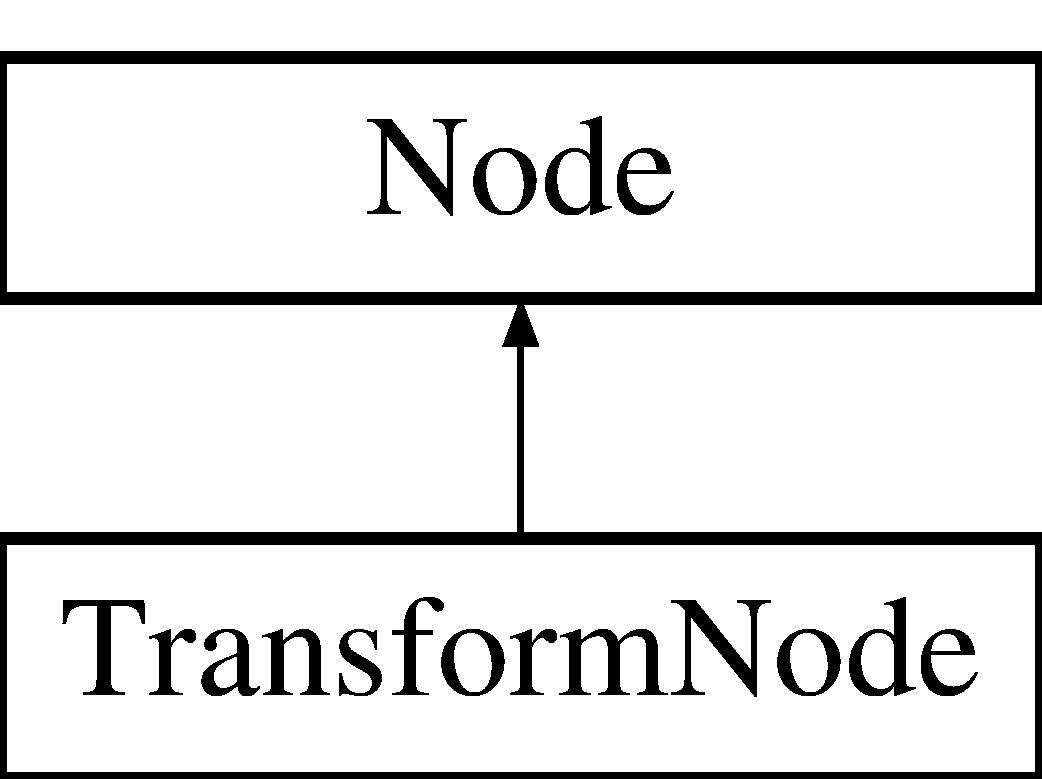
\includegraphics[height=2.000000cm]{classTransformNode}
\end{center}
\end{figure}
\subsection*{Public Member Functions}
\begin{DoxyCompactItemize}
\item 
\hypertarget{classTransformNode_aaf9b373c0d1b27b8fda450820ed52e69}{{\bfseries Transform\-Node} (const \hyperlink{classTransform}{Transform} \&t)}\label{classTransformNode_aaf9b373c0d1b27b8fda450820ed52e69}

\item 
void \hyperlink{classTransformNode_a746be4bb9fd24686ff2a6ad49c08c986}{execute} ()
\item 
\hypertarget{classTransformNode_ab73f2fb928f777deca2e093a7d909a71}{void {\bfseries set\-Parameters} (const Transform\-Type t, const G\-Lfloat $\ast$a)}\label{classTransformNode_ab73f2fb928f777deca2e093a7d909a71}

\end{DoxyCompactItemize}
\subsection*{Additional Inherited Members}


\subsection{Detailed Description}
Purpose\-: Wraps the \hyperlink{classTransform}{Transform} class with a node so it can be added to the scene. \begin{DoxyAuthor}{Author}
Andrew Dang-\/\-Tran 
\end{DoxyAuthor}


\subsection{Member Function Documentation}
\hypertarget{classTransformNode_a746be4bb9fd24686ff2a6ad49c08c986}{\index{Transform\-Node@{Transform\-Node}!execute@{execute}}
\index{execute@{execute}!TransformNode@{Transform\-Node}}
\subsubsection[{execute}]{\setlength{\rightskip}{0pt plus 5cm}void Transform\-Node\-::execute (
\begin{DoxyParamCaption}
{}
\end{DoxyParamCaption}
)\hspace{0.3cm}{\ttfamily [virtual]}}}\label{classTransformNode_a746be4bb9fd24686ff2a6ad49c08c986}
Applies the transform within the \hyperlink{classNode}{Node} to the matrix 

Reimplemented from \hyperlink{classNode_a6890991303fcc6c9b2b3dec678c8b5db}{Node}.



The documentation for this class was generated from the following files\-:\begin{DoxyCompactItemize}
\item 
Transform\-Node.\-h\item 
Transform\-Node.\-c++\end{DoxyCompactItemize}

\hypertarget{classTrimesh}{\section{Trimesh Class Reference}
\label{classTrimesh}\index{Trimesh@{Trimesh}}
}
\subsection*{Public Member Functions}
\begin{DoxyCompactItemize}
\item 
\hypertarget{classTrimesh_aee77f52567186fe071be314368a95a17}{void {\bfseries add\-Vertex} (const G\-Lfloat $\ast$coordinates)}\label{classTrimesh_aee77f52567186fe071be314368a95a17}

\item 
\hypertarget{classTrimesh_a38056e42e653cc58dcbd52f43db0ca75}{void {\bfseries add\-Face} (int $\ast$corner\-Indexes)}\label{classTrimesh_a38056e42e653cc58dcbd52f43db0ca75}

\item 
void \hyperlink{classTrimesh_aac7027d5aeb0af14e4503791e13d84fe}{calculate\-Normals} ()
\item 
void \hyperlink{classTrimesh_a817f3ec53aa8f052dcdb8c0cc54b0c4d}{render} (bool face\-Normal)
\item 
void \hyperlink{classTrimesh_ab05eecb8be123c1d1e65b94831a4c264}{render\-Normals} (bool face\-Normal, bool vertex\-Normal)
\end{DoxyCompactItemize}


\subsection{Member Function Documentation}
\hypertarget{classTrimesh_aac7027d5aeb0af14e4503791e13d84fe}{\index{Trimesh@{Trimesh}!calculate\-Normals@{calculate\-Normals}}
\index{calculate\-Normals@{calculate\-Normals}!Trimesh@{Trimesh}}
\subsubsection[{calculate\-Normals}]{\setlength{\rightskip}{0pt plus 5cm}void Trimesh\-::calculate\-Normals (
\begin{DoxyParamCaption}
{}
\end{DoxyParamCaption}
)}}\label{classTrimesh_aac7027d5aeb0af14e4503791e13d84fe}
Calculate the face and vertex normals of the mesh \hypertarget{classTrimesh_a817f3ec53aa8f052dcdb8c0cc54b0c4d}{\index{Trimesh@{Trimesh}!render@{render}}
\index{render@{render}!Trimesh@{Trimesh}}
\subsubsection[{render}]{\setlength{\rightskip}{0pt plus 5cm}void Trimesh\-::render (
\begin{DoxyParamCaption}
\item[{bool}]{face\-Normal}
\end{DoxyParamCaption}
)}}\label{classTrimesh_a817f3ec53aa8f052dcdb8c0cc54b0c4d}
Render the mesh 
\begin{DoxyParams}{Parameters}
{\em face\-Normal} & -\/ variable determining whether the normals are face normals or vertex normals. primarily affects lighting. \\
\hline
\end{DoxyParams}
\hypertarget{classTrimesh_ab05eecb8be123c1d1e65b94831a4c264}{\index{Trimesh@{Trimesh}!render\-Normals@{render\-Normals}}
\index{render\-Normals@{render\-Normals}!Trimesh@{Trimesh}}
\subsubsection[{render\-Normals}]{\setlength{\rightskip}{0pt plus 5cm}void Trimesh\-::render\-Normals (
\begin{DoxyParamCaption}
\item[{bool}]{face\-Normal, }
\item[{bool}]{vertex\-Normal}
\end{DoxyParamCaption}
)}}\label{classTrimesh_ab05eecb8be123c1d1e65b94831a4c264}
Render lines which represent the normals. 

The documentation for this class was generated from the following files\-:\begin{DoxyCompactItemize}
\item 
Geom.\-h\item 
Geom.\-c++\end{DoxyCompactItemize}

\hypertarget{classTrimeshLoader}{\section{Trimesh\-Loader Class Reference}
\label{classTrimeshLoader}\index{Trimesh\-Loader@{Trimesh\-Loader}}
}
\subsection*{Public Member Functions}
\begin{DoxyCompactItemize}
\item 
\hypertarget{classTrimeshLoader_a00499ce6cb6cd4f9f57d62ebabf23b22}{\hyperlink{structTokenPair}{Token\-Pair} $\ast$ {\bfseries token\-Match} (char $\ast$srchtok)}\label{classTrimeshLoader_a00499ce6cb6cd4f9f57d62ebabf23b22}

\item 
\hypertarget{classTrimeshLoader_a28a863ff38d4b4c6760efd42d9df86b2}{void {\bfseries load\-O\-B\-J} (const char $\ast$objfile, \hyperlink{classTrimesh}{Trimesh} $\ast$pmesh)}\label{classTrimeshLoader_a28a863ff38d4b4c6760efd42d9df86b2}

\item 
\hypertarget{classTrimeshLoader_a0da06aba10239fca53a38b44ea8b9a02}{int {\bfseries read\-Floats} (char $\ast$tok, float $\ast$buf, int bufsz)}\label{classTrimeshLoader_a0da06aba10239fca53a38b44ea8b9a02}

\item 
\hypertarget{classTrimeshLoader_a8e0ecbde14c2bb56824cf58dd4145168}{int {\bfseries read\-Ints} (char $\ast$tok, int $\ast$buf, int bufsz)}\label{classTrimeshLoader_a8e0ecbde14c2bb56824cf58dd4145168}

\item 
\hypertarget{classTrimeshLoader_a4af576992a8daadfa5122a94832ab6cd}{void {\bfseries process\-Skip} (char $\ast$tok)}\label{classTrimeshLoader_a4af576992a8daadfa5122a94832ab6cd}

\item 
\hypertarget{classTrimeshLoader_ad3b0d9cb78d5e9bc2c1b7deb0854da03}{void {\bfseries process\-Vertex} (char $\ast$tok, \hyperlink{classTrimesh}{Trimesh} $\ast$pmsh)}\label{classTrimeshLoader_ad3b0d9cb78d5e9bc2c1b7deb0854da03}

\item 
\hypertarget{classTrimeshLoader_a43b17b012e2a53f3ee21efb079ae9a01}{bool {\bfseries process\-Face} (char $\ast$tok, \hyperlink{classTrimesh}{Trimesh} $\ast$pmsh)}\label{classTrimeshLoader_a43b17b012e2a53f3ee21efb079ae9a01}

\end{DoxyCompactItemize}
\subsection*{Static Public Attributes}
\begin{DoxyCompactItemize}
\item 
\hypertarget{classTrimeshLoader_afbfd2f0835786c1a96423ebfe047d68a}{static \hyperlink{structTokenPair}{Token\-Pair} {\bfseries E\-M\-P\-T\-Y\-\_\-\-P\-A\-I\-R} =\{\char`\"{}\char`\"{},T\-\_\-\-N\-O\-N\-E\}}\label{classTrimeshLoader_afbfd2f0835786c1a96423ebfe047d68a}

\item 
static \hyperlink{structTokenPair}{Token\-Pair} {\bfseries token\-Map} \mbox{[}$\,$\mbox{]}
\item 
\hypertarget{classTrimeshLoader_a1ad0bd375daefe6b0989d0393a2bd516}{static char {\bfseries T\-O\-K\-\_\-\-S\-E\-P\-S} \mbox{[}$\,$\mbox{]} = \char`\"{} \textbackslash{}t\char`\"{}}\label{classTrimeshLoader_a1ad0bd375daefe6b0989d0393a2bd516}

\end{DoxyCompactItemize}


\subsection{Member Data Documentation}
\hypertarget{classTrimeshLoader_acc3b92a5900000c950c6aee14bea3569}{\index{Trimesh\-Loader@{Trimesh\-Loader}!token\-Map@{token\-Map}}
\index{token\-Map@{token\-Map}!TrimeshLoader@{Trimesh\-Loader}}
\subsubsection[{token\-Map}]{\setlength{\rightskip}{0pt plus 5cm}{\bf Token\-Pair} Trimesh\-Loader\-::token\-Map\hspace{0.3cm}{\ttfamily [static]}}}\label{classTrimeshLoader_acc3b92a5900000c950c6aee14bea3569}
{\bfseries Initial value\-:}
\begin{DoxyCode}
= \{ 
    \{\textcolor{stringliteral}{"v"}, T\_VERT\}, \{\textcolor{stringliteral}{"f"},T\_FACE\}, 
    EMPTY\_PAIR  
\}
\end{DoxyCode}


The documentation for this class was generated from the following files\-:\begin{DoxyCompactItemize}
\item 
Loader.\-h\item 
Loader.\-c++\end{DoxyCompactItemize}

\hypertarget{classVertex}{\section{Vertex Class Reference}
\label{classVertex}\index{Vertex@{Vertex}}
}


{\ttfamily \#include $<$Vertex.\-h$>$}

\subsection*{Public Member Functions}
\begin{DoxyCompactItemize}
\item 
\hypertarget{classVertex_aaeb85c70765a8a11cc54148054746129}{{\bfseries Vertex} (const G\-Lfloat $\ast$c=N\-U\-L\-L)}\label{classVertex_aaeb85c70765a8a11cc54148054746129}

\item 
\hypertarget{classVertex_a00ad86006f91af73121896906b2e0faa}{\hyperlink{classVertex}{Vertex} \& {\bfseries operator=} (const \hyperlink{classVertex}{Vertex} \&)}\label{classVertex_a00ad86006f91af73121896906b2e0faa}

\item 
void \hyperlink{classVertex_a437201cc8e7ae5b8f49f47fe9dd4beba}{contribute\-Normal} (const G\-Lfloat $\ast$n)
\item 
void \hyperlink{classVertex_a8ab3c20d57d0626ebbc15271376a7a8d}{average\-Normals} ()
\item 
\hypertarget{classVertex_a5b5b877aedb2ca726643302fe440ca19}{void {\bfseries draw\-Normal} () const }\label{classVertex_a5b5b877aedb2ca726643302fe440ca19}

\item 
\hypertarget{classVertex_a17aebadfb3748f956ddf098b171c09ca}{G\-Lfloat $\ast$ {\bfseries get\-Normal} ()}\label{classVertex_a17aebadfb3748f956ddf098b171c09ca}

\item 
\hypertarget{classVertex_af674e1c88da20e86a18a7e06370eac5d}{const G\-Lfloat $\ast$ {\bfseries get\-Const\-Normal} () const }\label{classVertex_af674e1c88da20e86a18a7e06370eac5d}

\item 
\hypertarget{classVertex_a5963c45ed490edba17cb4e0030e6781e}{const G\-Lfloat $\ast$ {\bfseries get\-Coordinates} () const }\label{classVertex_a5963c45ed490edba17cb4e0030e6781e}

\item 
const int \hyperlink{classVertex_ad378995fa3c86a6d37e7746c7cb6873e}{get\-Num\-Faces} () const 
\end{DoxyCompactItemize}


\subsection{Detailed Description}
Purpose\-: Class stores vertex information for meshes \begin{DoxyAuthor}{Author}
Andrew Dang-\/\-Tran 
\end{DoxyAuthor}


\subsection{Member Function Documentation}
\hypertarget{classVertex_a8ab3c20d57d0626ebbc15271376a7a8d}{\index{Vertex@{Vertex}!average\-Normals@{average\-Normals}}
\index{average\-Normals@{average\-Normals}!Vertex@{Vertex}}
\subsubsection[{average\-Normals}]{\setlength{\rightskip}{0pt plus 5cm}void Vertex\-::average\-Normals (
\begin{DoxyParamCaption}
{}
\end{DoxyParamCaption}
)}}\label{classVertex_a8ab3c20d57d0626ebbc15271376a7a8d}
Average the normals of all the connecting faces of this vertex. \hypertarget{classVertex_a437201cc8e7ae5b8f49f47fe9dd4beba}{\index{Vertex@{Vertex}!contribute\-Normal@{contribute\-Normal}}
\index{contribute\-Normal@{contribute\-Normal}!Vertex@{Vertex}}
\subsubsection[{contribute\-Normal}]{\setlength{\rightskip}{0pt plus 5cm}void Vertex\-::contribute\-Normal (
\begin{DoxyParamCaption}
\item[{const G\-Lfloat $\ast$}]{n}
\end{DoxyParamCaption}
)}}\label{classVertex_a437201cc8e7ae5b8f49f47fe9dd4beba}
Add the normal of a face to the vertex \hypertarget{classVertex_ad378995fa3c86a6d37e7746c7cb6873e}{\index{Vertex@{Vertex}!get\-Num\-Faces@{get\-Num\-Faces}}
\index{get\-Num\-Faces@{get\-Num\-Faces}!Vertex@{Vertex}}
\subsubsection[{get\-Num\-Faces}]{\setlength{\rightskip}{0pt plus 5cm}const int Vertex\-::get\-Num\-Faces (
\begin{DoxyParamCaption}
{}
\end{DoxyParamCaption}
) const}}\label{classVertex_ad378995fa3c86a6d37e7746c7cb6873e}
Return the number of faces which is connected to this vertices 

The documentation for this class was generated from the following files\-:\begin{DoxyCompactItemize}
\item 
Vertex.\-h\item 
Vertex.\-c++\end{DoxyCompactItemize}

%--- End generated contents ---

% Index
\newpage
\phantomsection
\addcontentsline{toc}{chapter}{Index}
\printindex

\end{document}
